%% Copernicus Publications Manuscript Preparation Template for LaTeX Submissions
%% ---------------------------------
%% This template should be used for copernicus.cls
%% The class file and some style files are bundled in the Copernicus Latex Package, which can be downloaded from the different journal webpages.
%% For further assistance please contact Copernicus Publications at: production@copernicus.org
%% https://publications.copernicus.org/for_authors/manuscript_preparation.html


%% Please use the following documentclass and journal abbreviations for discussion papers and final revised papers.

%% 2-column papers and discussion papers
\documentclass[acp]{copernicus}



%% Journal abbreviations (please use the same for discussion papers and final revised papers)


% Advances in Geosciences (adgeo)
% Advances in Radio Science (ars)
% Advances in Science and Research (asr)
% Advances in Statistical Climatology, Meteorology and Oceanography (ascmo)
% Annales Geophysicae (angeo)
% Archives Animal Breeding (aab)
% ASTRA Proceedings (ap)
% Atmospheric Chemistry and Physics (acp)
% Atmospheric Measurement Techniques (amt)
% Biogeosciences (bg)
% Climate of the Past (cp)
% DEUQUA Special Publications (deuquasp)
% Drinking Water Engineering and Science (dwes)
% Earth Surface Dynamics (esurf)
% Earth System Dynamics (esd)
% Earth System Science Data (essd)
% E&G Quaternary Science Journal (egqsj)
% European Journal of Mineralogy (ejm)
% Fossil Record (fr)
% Geochronology (gchron)
% Geographica Helvetica (gh)
% Geoscience Communication (gc)
% Geoscientific Instrumentation, Methods and Data Systems (gi)
% Geoscientific Model Development (gmd)
% History of Geo- and Space Sciences (hgss)
% Hydrology and Earth System Sciences (hess)
% Journal of Micropalaeontology (jm)
% Journal of Sensors and Sensor Systems (jsss)
% Magnetic Resonance (mr)
% Mechanical Sciences (ms)
% Natural Hazards and Earth System Sciences (nhess)
% Nonlinear Processes in Geophysics (npg)
% Ocean Science (os)
% Primate Biology (pb)
% Proceedings of the International Association of Hydrological Sciences (piahs)
% Scientific Drilling (sd)
% SOIL (soil)
% Solid Earth (se)
% The Cryosphere (tc)
% Weather and Climate Dynamics (wcd)
% Web Ecology (we)
% Wind Energy Science (wes)


%% \usepackage commands included in the copernicus.cls:
%\usepackage[german, english]{babel}
%\usepackage{tabularx}
%\usepackage{cancel}
%\usepackage{multirow}
%\usepackage{supertabular}
%\usepackage{algorithmic}
%\usepackage{algorithm}
%\usepackage{amsthm}
%\usepackage{float}
%\usepackage{subfig}
%\usepackage{rotating}
% \usepackage{ce}

\newcommand{\uOPm}{\unit{nmol~min^{-1}~µg^{-1}}}
\newcommand{\uOPv}{\unit{nmol~min^{-1}~m^{-3}}}
\newcommand{\uPMconc}{\unit{µg~m^{-3}}}
\hypersetup{
    colorlinks,breaklinks,   % deleted ps2pdf 11/6/15
    linkcolor=blue,
    urlcolor=red,
    citecolor=blue,
    hyperfootnotes=false,
}

\begin{document}

\title{
Source apportionment of the oxidative potential of aerosols at 15 French
sites for yearly time series of observation
}


% \Author[affil]{given_name}{surname}

\Author[1]{Samuël}{Weber}
\Author[1]{Gaëlle}{Uzu}
\Author[1]{Aude}{Calas}
\Author[1]{Dalia}{Salameh}
\Author[1]{Florie}{Chevrier}
\Author[1]{Julie}{Allard}
\Author[2]{Jean-Luc}{Besombes}
\Author[3]{Alexandre}{Albinet}
\Author[3]{Olivier}{Favez}
\Author[4,5,6,7,8]{les}{AASQA}
\Author[1]{Jean-Luc}{Jaffrezo}

\affil[1]{Univ. Grenoble Alpes, CNRS, IRD, IGE (UMR 5001), 38000 Grenoble, France}
\affil[2]{Univ. Savoie Mont Blanc, LCME, 73000 Chambéry, France}
\affil[3]{INERIS, Parc Technologique Alata, BP 2, 60550 Verneuil-en-Halatte, France}
\affil[4]{Atmo AuRA, 69500 Bron, France}
\affil[5]{Atmo Sud, 13294 Marseille, France}
\affil[6]{Atmo Hauts de France, 59044 Lille, France}
\affil[7]{Atmo Nouvelle Aquitaine, 33692 Merignac, France}
\affil[8]{Atmo Grand Est, 57070 Metz, France}


%% The [] brackets identify the author with the corresponding affiliation. 1, 2, 3, etc. should be inserted.

%% If an author is deceased, please mark the respective author name(s) with a dagger, e.g. "\Author[2,$\dag$]{Anton}{Aman}", and add a further "\affil[$\dag$]{deceased, 1 July 2019}".

%% If authors contributed equally, please mark the respective author names with an asterisk, e.g. "\Author[2,*]{Anton}{Aman}" and "\Author[3,*]{Bradley}{Bman}" and add a further affiliation: "\affil[*]{These authors contributed equally to this work.}".



\correspondence{NAME (EMAIL)}

\runningtitle{Source apportionement of OP in France}

\runningauthor{S. Weber et al.}




\received{}
\pubdiscuss{} %% only important for two-stage journals
\revised{}
\accepted{}
\published{}

%% These dates will be inserted by Copernicus Publications during the typesetting process.


\firstpage{1}

\maketitle



\begin{abstract}

The reactive oxygen species (ROS) carried or induced by particulate
matter (PM) are suspected to induce oxidative stress in vivo, leading to
health impacts in Human populations. The oxidative potential (OP) of PM,
displaying the ability of PM to oxidize the lung environment is gaining
a strong interest to examine health risks associated to PM exposure. In
this study, OP was measured by two different acellular assays
(dithiothreitol, DTT and ascorbic acid, AA) on samples from yearly time
series of filters collected in 15 different sites in France between 2013
and 2016, including urban, traffic and valley typologies. The same
filters were characterized with an advanced chemical speciation allowing
source-apportionment of PM\textsubscript{10} using positive matrix
factorization PMF method for each series, for a total above 1700
samples. This study provides therefore a nation-wide synthesis on the
source-apportionment of OP using coupled PMF and multiple linear
regression model. The road traffic, biomass burning, dust, MSA-rich, and
primary biogenic sources have distinct positive redox-activity towards
the OP\textsuperscript{DTT} assay. The OP\textsuperscript{AA} assay only
presents significant activity for the biomass burning and road traffic
sources. The daily median source contribution to the total
OP\textsubscript{DTT} highlights the dominant influence of the road
traffic source. Both the biomass burning and the road traffic sources
contribute evenly to the observed OP\textsuperscript{AA}. Would the OP
being a good proxy of Human health impact, it appears that domestic
biomass burning and road traffic are the two main sources to target in
order to decrease significantly the OP over the French territory and to
lower the health risks from PM exposure.

\end{abstract}


\copyrightstatement{TEXT}




\introduction%% \introduction[modified heading if necessary]

Air quality has become a major public health issue, being the fourth global cause of
mortality with 7 million premature deaths worldwide per year due to both indoor and
outdoor exposure~\citep{worldhealthorganizationAmbient2016}.  Driving 90 \% of this health
impact~\citep{lelieveldContribution2015}, particulate matter (PM) is one of the key
pollutants in the air linked to health outcomes, although the exact mechanism leading to
toxicity is not yet fully
understood~\citep{barraza-villarrealAir2008,beck-speierUltrafine2012,brauerExposure2012,goixEnvironmental2014,goldbergSystematic2011,salehExposure2019}.
Many urbanized areas, mainly located in low- or middle-incomes countries, are exposed to
PM concentration far higher than the recommendation guideline of the WHO.

Although PM are now monitored in many countries and large efforts are
observed to document ambient concentrations, the underlying processes
leading to the observed concentrations in the atmosphere, and
particularly the understanding of emissions sources, are still an active
field of
research~\citep{diemozTransport2019,elhaddadPrimary2011,gollyOrganic2019,hodshirePotential2019,jaffrezoSeasonal2005,jiangSources2019,marconiSaharan2014,morenoVariations2010,piotQuantification2012,salamehPM22015,samakePolyols2019,wakedSource2014}.
In recent years, strong focus has been put worldwide on
source-apportionment methods in order to better understand the processes
leading to the airborne concentrations and the accumulation of PM in the
atmosphere. This includes direct modeling approaches such as Chemistry
Transport Model using tagged
species~\citep{brandtContribution2013,kranenburgSource2013,mirceaEuropean2020,wagstromDevelopment2008,wangDevelopment2009}
or field studies coupled with receptor models
(RM)~\citep{belisEvaluation2020,pernigottiSPECIEUROPE2016,simonDevelopment2010}, notably Positive
Matrix Factorization (PMF). PMF can be based either on AMS time resolve
spectrum~\citep{bozzettiArgon2017,petitSubmicron2014,petitTwo2015} or on filter
analysis~\citep{amatoAIRUSELIFE2016,bressiSources2014,fangPM22015,jainSource2018,jainSeasonal2020,liuSource2016,petitSources2019,salamehSources2018,srivastavaSpeciation2018a,wakedSource2014}
or a mix of these different measurement
techniques~\citep{costabileFirst2017,vlachouAdvanced2018,vlachouDevelopment2019}.
Score of results indicate that PM originate from a
wide variety of sources, not only from natural (volcano, sea spray, soil
dust, vegetation, bacteria, pollen\ldots) or anthropogenic (road
traffic, residential heating, industry\ldots) sources, but also is
formed as secondary product and condensed from the gaseous phase
(ammonium-nitrate and -sulfate\ldots). As a result, the chemistry, size
distribution or reactivity of PM widely vary from location to location
and season to season, which induces large changes in the health impacts
depending on all of these parameters~\citep{kellySize2012}.

Faced with this diversity, it is understandable that epidemiological
studies have difficulty in finding clear links between the atmospheric
mass concentration of PM and the associated short-term health impacts.
Indeed, the mass of PM may not be the relevant metric when dealing with
health impacts of airborne particles since major properties (chemistry,
shape, size distribution, solubility, speciation) driving PM toxicity
are not taken into account within the mass. It is now believed that the
measurement of the reactive oxygen species (ROS) should be more closely
linked to the potential adverse health effects of atmospheric PM, since
oxidative stress is a key factor in the inflammatory response of the
organism, leading for instance to respiratory diseases or when exposed
for a long period of time, cardiovascular diseases or even
cancer~\citep{lelieveldContribution2015,liParticulate2003a}. Therefore, the
oxidizing potential (OP) of PM being an indirect measure of the ability
of the particles to induce ROS in a biological
medium~\citep{ayresEvaluating2008,choRedox2005,liOxidant2009,sauvainNanoparticle2008}
has been proposed as a potential proxy of the health impacts of atmospheric
exposure. Indeed, some recent studies already established associations
between OP and different possible health
outcomes~\citep{costabileEvidence2019,karavalakisImpact2017,steenhofVitro2011,strakAssociations2017,tuetChemical2017,weichenthalFine2016,weichenthalOxidative2016}

The demonstration of the OP to be a good proxy of health impact is still
needed. At this point, tThere is also no clear consensus toward a
standardized method to measure the OP of PM, and many assays and
protocols co-exist (DTT, GSH, AA, ESR, °OH or
H\textsubscript{2}O\textsubscript{2}, among others), with samples
extracted with different methods (water, simulated lung fluid (SLF),
etc.)., and not always with a constant mass of PM. However, the
dithiothreitol (DTT) and ascorbic-acid (AA) assay are widely used in
associations with health
endpoints~\citep{abramsAssociations2017,atkinsonShortterm2016,batesReactive2015,canovaPM102014,fangOxidative2016,janssenAssociations2015,strakLongterm2017,weichenthalOxidative2016,yangChildren2016,zhangAssociations2016}
even if the exact methodologies
differ from one study to the other. The same is true for the seasonality
of OP based on these two
assays~\citep{batesReactive2015,calasSeasonal2019,cesariSource2019,fangOxidative2016,maSources2018,paraskevopoulouYearlong2019,perronePM2016,pietrograndeChemical2018,vermaReactive2014,vermaOrganic2015,weberApportionment2018,zhouPredominance2019}.
Finally, several studies also linked OP variabilities with the contributions of
emission sources of PM (references) Several studies have already shown
that different sources of PM have different reactivity to OP
tests~\citep{batesReactive2015,cesariSource2019,fangOxidative2016,paraskevopoulouYearlong2019,vermaReactive2014,weberApportionment2018,zhouPredominance2019}. In particular, sources with high concentrations of
transition metals, such as road traffic, appear to have a higher
intrinsic oxidizing potential than other sources of PM., even if the
exact methodologies differ from one study to the other.

Thus, it is now necessary to know if this new parameter of PM (oxidizing
potential) complements the usual metric (mass concentration per cubic
meter).

Several studies have already shown that different sources of PM have
different reactivity to OP
tests~\citep{batesReactive2015,cesariSource2019,fangOxidative2016,paraskevopoulouYearlong2019,vermaReactive2014,weberApportionment2018,zhouPredominance2019}. In particular, sources
with high concentrations of transition metals, such as road traffic,
appear to have a higher intrinsic oxidizing potential than other sources
of PM. However, the studies in question are still rare and do not always
take into account complete seasonal cycles and therefore may not
encompass the variety of sources for a given site omitting some
important sources. Also, spatial variability at the country-scale is
currently unknown and requires homogeneous sampling and analysis
methodologies for all filters and time-series.

In order to address these questions, we gathered in this study an
extensive database of about 1 700 samples from 15 yearly time-series of
observations over continental France, collected during many research
programs conducted between 2013 and 2018. On each of these samples, we
concurrently measured the OP with the DTT and AA assays, together with
an extensive chemical characterization allowing PM source apportionment
using a harmonized PMF (Positive Matrix Factorization)
approach~\citep{weberComparison2019}. Then, we apportioned the OP measured by the DTT and AA
assay to the emission sources using a multilinear regression approach,
following~\citet{weberApportionment2018}. In this way, we can estimate the
oxidizing capacity of each microgram of PM from the different identified
emission sources but also the relative contribution of the different
sources to the OP\textsuperscript{DTT} and OP\textsuperscript{AA} on
seasonal and daily basis.

\section{Material and method}%
\label{material_and_method}

\subsection{Sites description}%
\label{sites_description}

The selected sites had to fulfill three conditions: 1) a yearly sampling
period, 2) the required chemical analysis to perform a standardized PMF
study and 3) enough filter surface left to assess the OP measurements. A
total of 14 sites were included in this study (one being sampled 2 times
at 5 years interval) taken from different research programs. The chosen
sites reflect the diversity of typology we could encounter in the
western Europe: urban (NGT, TAL, AIX, MRS-5av), urban traffic (NIC),
urban alpine valley (GRE-cb, GRE-fr, VIF, CHAM, MNZ, PAS), industrial
(PdB) and traffic (RBX \& STG-ce) and are details in
Table~\ref{tab:tab1} and cover different
area of France (Figure~\ref{fig:fig1}).
All these sites are monitored by the local AASQA (Atmo Sud, Atmo AURA,
Atmo Aquitaine and Atmo HdF). We note, however, the absence of remote or
rural sites in our current dataset.

\begin{figure*}[ht]
    \centering
    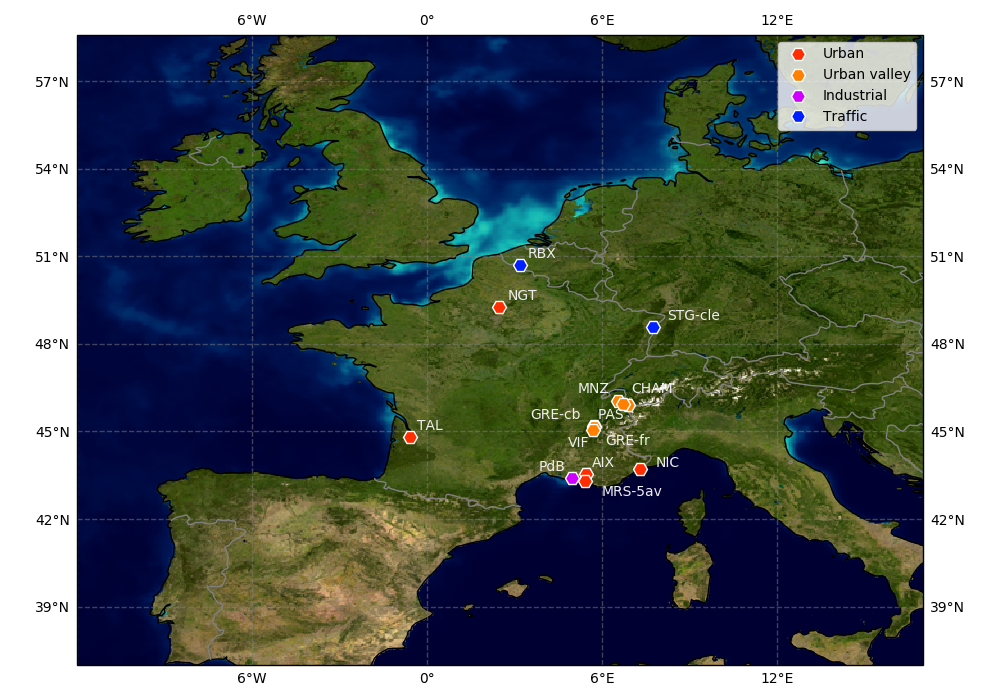
\includegraphics[width=0.7\linewidth]{figures/fig1}
    \caption{
    Location of the 15 sampling sites. Color codes denote the typology of the
    site: red, urban; orange, urban valley; magenta, industrial; blue, traffic.
    }%
    \label{fig:fig1}
\end{figure*}

\begin{table*}[ht]
    \centering
    \caption{
     Sampling sites meta-data.
    }
    \label{tab:tab1}
    \begin{tabular}{lllllll}
\tophline
Ville           & Abbreviation & Typology      & Coordinate            & Elevation & \# sample & Date\\
\middlehline
Marseille       & MRS-5av      & Urban bgd     & 43.3060 °N, 5.3957 °E & 64 m   & 72  & 2015-01-11 → 2015-12-28\\
Port-de-Bouc    & PdB          & Industrial    & 43.4019 °N, 4.9819 °E & 1 m    & 113 & 2014-06-01 → 2015-05-17\\
Aix-en-provence & AIX          & Urban bgd     & 43.5302 °N, 5.4413 °E & 188 m  & 56  & 2013-08-02 → 2014-07-13\\
Nice            & NIC          & Urban traffic & 43.7020 °N, 7.2862 °E & 1 m    & 105 & 2014-07-11 → 2015-05-26\\
Talence         & TAL          & Urban bgd     & 44.8004 °N, 0.5880 °W & 20 m   & 120 & 2012-03-01 → 2013-03-19\\
Nogent          & NGT          & Urban bgd     & 49.2763 °N, 2.4821 °E & 28 m   & 135 & 2013-01-02 → 2014-05-11\\
Grenoble        & GRE-fr\_2013 & Urban bgd     & 45.1618 °N, 5.7356 °E & 214 m  & 225 & 2013-01-02 → 2014-12-29\\
Grenoble        & GRE-fr\_2017 & Urban bgd     & 45.1618 °N, 5.7356 °E & 214 m  & 122 & 2017-02-28 → 2018-03-10\\
Grenoble        & GRE-cb       & Urban bgd     & 45.1833 °N, 5.7251 °E & 212 m  & 124 & 2017-02-28 → 2018-03-10\\
Vif             & VIF          & Urban bgd     & 45.0580 °N, 5.6768 °E & 310 m  & 125 & 2017-02-28 → 2018-03-10\\
Chamonix        & CHAM         & Urban valley  & 45.9225 °N, 6.8699 °E & 1038 m & 93  & 2013-11-02 → 2014-10-31\\
Marnaz          & MNZ          & Urban valley  & 46.0577 °N, 6.5334 °E & 504 m  & 89  & 2013-11-02 → 2014-10-31\\
Passy           & PAS          & Urban valley  & 45.9235 °N, 6.7136 °E & 588 m  & 88  & 2013-11-02 → 2014-10-31\\
Roubaix         & RBX          & Traffic       & 50.7065 °N, 3.1806 °E & 10 m   & 157 & 2013-01-20 → 2014-05-26\\
Strasbourg      & STG-cle      & Traffic       & 48.5903 °N, 7.7450 °E & 139 m  & 76  & 2013-04-11 → 2014-04-08\\
\bottomhline
    \end{tabular}
\belowtable{bgd: background} % Table Footnotes
\end{table*}

\subsection{Sample analysis}%
\label{sample-analysis}

\subsubsection{Chemical speciation}%
\label{chemical-speciation}

The PM\textsubscript{10} concentration was measured at each site by
means of an automatic analyzer, according to EN 16450:2017~\citep{cenAmbient2017},
and daily (24~hours) filter samples were collected every third day by
employees of the corresponding regional air quality monitoring network.
Samplings were achieved on pre-heated quartz fiber filters using
high-volume sampler (DA80, Digitel), following EN 12341:2014
procedures~\citep{cenAmbient2014}. Off-line chemical analysis performed on these
filters are fully described in the respective papers. Briefly, the
elemental and organic carbon fractions (EC and OC) were measured via
thermo-optical analysis (Sunset Lab. Analyzer~\citep{birchElemental1996})
using the EUSAAR-2 protocol~\citep{cavalliStandardised2010,cenAmbient2017a}. Major
water-soluble inorganic contents (Cl\textsuperscript{-},
NO\textsubscript{3}\textsuperscript{-},
SO\textsubscript{4}\textsuperscript{2-} ,
NH\textsubscript{4}\textsuperscript{+}, Na\textsuperscript{+},
K\textsuperscript{+}, Mg\textsuperscript{2+}, and
Ca\textsuperscript{2+}) and methanesulfonic acid (MSA) were determined
using ion chromatography~\citep{cenAmbient2017b,jaffrezoSize2005}. Many
metals or trace elements (e.g., Al, Ca, Fe, K, As, Ba, Cd, Co, Cu, La,
Mn, Mo, Ni, Pb, Rb, Sb, Sr, V, and Zn) were measured by ICP-AES or
ICP-MS~\citep{allemanPM102010,mbengueSizedistributed2014,cenAmbient2005}. Finally,
various anhydrosugars (including levoglucosan, mannosan, arabitol,
sorbitol, and mannitol) were analyzed using High Performance Liquid
Chromatography followed by pulsed amperometric detection
(HPLC-PAD)~\citep{wakedSource2014}.

\subsubsection{OP assays}%
\label{op-assays}

The same methodology was applied for all the OP measurements of the
collected filters~\citep{calasImportance2017,calasComparison2018,calasSeasonal2019}. Shortly, we
performed the extraction of PM into a simulated lung fluid (SLF) to
simulate the bio-accessibility of PM and to closely simulate exposure
conditions. In order to take into account the non-linearity of the OP
with the mass and to have comparable results between them, the
extraction takes place at iso-mass (10 or 25 of PM, depending on the
site), by adjusting the area of filter extracted. The filter extraction
method includes both water soluble and insoluble species. After the SLF
extraction, particles removed from filter are not filtrated, the whole
extract is injected in the multi-wall plate. Samples were processed
using the AA and DTT assays. DTT depletion when in contact with PM
extracts was determined by dosing the remaining amount of DTT with DTNB
(dithionitrobenzoic acid) at different reaction times (0, 15, 30
minutes) and absorbency was measured at 412~nm using a plate
spectrophotometer (Tecan, M200 Infinite). The AA assay is a simplified
version of the synthetic respiratory tract lining fluid (RTFL)
assay~(Kelly and Mudway, 2003), where only AA is used. AA depletion is
read continuously for 30 minutes by absorbency at 265 nm~ (TECAN, M1000
Infinite). The maximum depletion rate of AA is determined by linear
regression of the linear section data. For both assays, the 96-wells
plate is auto shaken for 3 seconds before each measurement and kept at
37° C~. Three filter blanks (laboratory blanks) and three positive
controls (1,4 Napthoquinone, 24,7 µM~) are included in every plate
(OP\textsuperscript{AA} and OP\textsuperscript{DTT}) of the protocol.
The average values of these blanks are then subtracted from the sample
measurement of this plate. Detection limit (DL) value is defined as
three times of the standard deviation of laboratory blanks measurements
(blank filters in Gamble+DPPC solution).

The samples were stored from 1 to 4 years before they were analyzed for
the DECOMBIO and SOURCES sites. The MobilAir samples were analyzed in
the months following their collection. As mentioned in \citet{vermaFractionating2015}, the
OP activity may be impacted by such storage time. However, in
a previous program \citep{ansesexposureEtude2017}, still ongoing, we have been
measuring the same filter over time. Over one year (about one
measurement per month), OP results for DTT and AA assays display
respectively a coefficient of variation of 18 and 12 \%. Hereafter, the
OP\textsuperscript{DTT} and OP\textsuperscript{AA} normalized by air
volume are noted OP\textsubscript{v}\textsuperscript{DTT} and
OP\textsubscript{v}\textsuperscript{AA}, respectively, with unit .

\subsection{Source apportionment}%
\label{source-apportionment}

The source apportionment of the OP can be performed in two main ways: 1)
include the OP as an input variable for receptor-model
(RM)~\citep{cesariSource2019,fangOxidative2016,maSources2018,vermaReactive2014}
or 2) conduct source attribution to the PM mass and then, using a multiple
linear regression (MLR) model, assign OP to each of the sources from the
source-receptor
model~\citep{batesReactive2015,cesariSource2019,paraskevopoulouYearlong2019,vermaOrganic2015,weberApportionment2018,zhouPredominance2019}.
We decided to use the second approach because the
inclusion of OP in the PMF could potentially destabilize the results but
also forces the OP to positive values (see below).

\subsubsection{PM mass apportionment: Positive Matrix Factorization}%
\label{pm-mass-apportionment-positive-matrix-factorization}

\paragraph{Methodological background}%
\label{methodological-background}

The source apportionment at the 15 sites was conducted thanks to a
Positive Matrix Factorization (PMF), using the EPA PMF 5.0
software~\citep{usepaPositive2017}
that makes use of the ME-2 solver from~\citet{paateroMultilinear1999}.
Briefly, the PMF was introduced by~\citet{paateroPositive1994} and is now
a common tool for source-apportionment study. It aims at solving the
receptor model equation
\begin{align}
    X &= G \cdot F,
\end{align}
where \(X\) is the \emph{n×m} observation matrix, \(G\) is the
\emph{n×p} contribution matrix and \(F\) is the \emph{p×m} factor
profile (or \emph{source}, but some factor are not a proper emission
\emph{source} but may reflect secondary processes), with \emph{n} the
number of sample, \emph{m} the number of measured chemical specie and
\emph{p} the number of profile. Hereafter, the \(G\) matrix will be in
and the \(F\) matrix in of PM.

\paragraph{PMF set up}%
\label{pmf-set-up}

Some of the PMFs were run during previous campaign, namely
SOURCES~({\url{http://pmsource.u-ga.fr}},~\citet{favezTraitement2017,weberComparison2019}),
DECOMBIO~\citep{chevrierChauffage2016,chevrierDECOMBIOContribution2016}, MobilAir
(\url{https://mobilair.univ-grenoble-alpes.fr/},~\citet{borlazaFinescaleinprep.}).
For the aims of this study, all PMF have been rerun according to a
harmonized methodology, following the SOURCES program, in order to have
a common set of input species and constraints in the model and to have
comparable sources' profiles.

The input species are slightly site-dependent, but include carbonaceous
compound (OC \& EC), ions (SO\textsubscript{4}\textsuperscript{2-},
NO\textsubscript{3}\textsuperscript{-}, Cl\textsuperscript{-},
NH\textsubscript{4}\textsuperscript{+}, K\textsuperscript{+},
Mg\textsuperscript{2+}, Ca\textsuperscript{2+}), organic compounds
(levoglucosan, mannosan, arabitol, manitol (summed and referred to
polyols) and MSA) and metals for a total of about 30 species. The list
of metals is not exactly the same for each of the sites, due to too low
concentrations on some filters. The uncertainties were estimated thanks
to the method proposed by~\citet{gianiniComparative2012} and was tripled if the
signal over noise ratio was below 2 (classified as ``weak'' in the PMF
software). Between 8 to 10 factors were identified for at the different
sites and are summarized in Table SI REF. On each of the PMF, the
possibility of adding constraints to the factors was used to better
disentangle possible mixing between factors and reduce the rotational
ambiguity, based on \emph{a priori} expert knowledge of the sources
geochemistry. A PMF solution was considered valid if it followed the
recommendation of the European guide on air pollution source
apportionment with receptor models~(Belis et al., 2019) as well as the
geochemical identification of the various factors. Estimation of the
precision of the PMF was obtained on both the base and constrained runs
thanks the both the bootstrap (BS) and displacement (DISP) functions of
the EPA PMF5.0.

\subsection{Similarity assessment of the PMF factors}%
\label{similarity-assessment-of-the-pmf-factors}

Since PMF resolves sites-specific factor of PM, we may question if a
factor named by the user ``Primary traffic'' at CHAM display indeed a
similar chemistry as a ``Primary traffic'' at NGT for instance. In order
to identify the the chemical similarity of the PMF profiles, a
similarity assessment of all PMF factor profiles was run following the
DeltaTool approach~\citep{pernigottiDeltaSA2018}, similarly to what we
presented recently in~\citet{weberComparison2019}. Shortly, the DeltaTool
approach compares a pair of factor profile based on it mass-normalized
chemical compounds thanks to 2 different metrics, the Pearson distance
(PD) and the standardized identity distance (SID) 
(see~\citet{belisNew2015a} for a detailed explanation of theses 2 metrics). The first one
is 1 minus the Pearson correlation coefficient
(\(\text{PD} = 1 - r^{2}\)) and so is strongly influenced by individual
extreme points (namely OC or EC in our dataset) whereas the second one,
SID, is more sensitive to every specie since it includes a normalization
term, expressed as follows
\begin{align}
    \text{SID} &= \frac{\sqrt{2}}{m}\sum_{j = 1}^{m}\frac{\left| x_{j} - y_{j} \right|}{x_{j} + y_{j}},
\end{align}
where \emph{x} and \emph{y} are two different factors profile in
relative mass and \emph{m} the number of common specie in \emph{x} and
\emph{y}.

\subsection{OP apportionment}%
\label{op-apportionment}

\subsubsection{Multiple linear inversion}%
\label{multiple-linear-inversion}

Similar to~\citet{weberApportionment2018}, a multiple linear regression (MLR) was
conducted independently at each sites with the two OP (DDT and AA) being
the dependent variables and the sources contribution obtained from the
PMF being the explanatory variables, following the equation:
\begin{align}
    \text{OP}_{\text{obs}} &= G \times \beta + \varepsilon,
\end{align}
with \emph{OP\textsubscript{obs}} a vector of size \emph{n×1} of the
observed OP\textsubscript{v}\textsuperscript{DTT} or
OP\textsubscript{v}\textsuperscript{AA} in , \(G\) is the matrix
(\emph{n×(p+1)}) of the mass contribution of PM sources determined from
the PMF in and a constant unit term for the intercept (no unit),
\emph{$\beta$} the coefficients (i.e. intrinsic OP of the source and the
intercept) of size (\emph{(p+1)×1}) in for the intrinsic OP and for the
intercept. The residual term \emph{$\varepsilon$} (\emph{n×1}) accounts for the
misfit between the observation and the model. We expressively did not
fix the intercept to zero. Indeed, if the system is well constrained the
intercept should be close to zero and conversely a non-zero intercept
would point out missing explanatory variables. A weighted least square
(WLS) were used in order to take into account the uncertainties of the
OP measurements.

In our previous study, we used a stepwise backward
elimination of negative coefficients.The assumption was that air is an
oxidative environment, thus the PM oxidative potential cannot be
negative. However, the application of this method to our enlarged
dataset led, at some sites, to unrealistic exclusion of almost all
sources together with a bad reconstruction of OP. This observation tends
in favor of possible coating effect of some oxidative species in
presence of other chemical components or non-linear effects, seen in our
model as ``negative'' OP. We then decided to remove the positivity
constraint in this study. Moreover, the removal of this constraint lead
to more homogeneous intrinsic OP for the main PM sources.

A careful data-treatment was performed in order to remove from the
dataset highly specific samples (e.g. firework) since we focus in this
study to the dominant sources and processes leading to the population
exposure of OP.

The uncertainties of the coefficients $\beta$ given by the MLR were estimated
by bootstrapping (BS) the solutions 500 times with randomly selected 70
\% of the samples in order to account for possible extremes events or
seasonal variations of the intrinsic OP per source. The uncertainty of
the PMF result G is not taken into account.

The computation was done thanks to the WLS method of the
\emph{statsmodels} package of python~\citep{seaboldStatsmodels2010}.

\subsubsection{Contribution of the sources to the OP}%
\label{contribution-of-the-sources-to-the-op}

The contribution G\textsuperscript{OP} in of the sources to the OP is
computed at each site independently and is simply the product of the
intrinsic OP $\beta$ in from the MLR times the source contribution of the PMF
G in :
\begin{align}
    G_{k}^{\text{OP}} &= G_{k} \times \beta_{k}
\end{align}
where \emph{k} is the source considered. The uncertainties of
G\textsuperscript{OP} is computed thanks to the uncertainties of $\beta$
estimated from the BS. The uncertainties of the PMF G\textsubscript{k}
is not taken into account.

\section{Results}%
\label{results}

Due to the amount of results, unlikely to be summarized into single
graph, we also present an interactive visualization of all the results
at \href{http://getopstandop.u-ga.fr/}{http://getopstandop.u-ga.fr}
where the reader can find all the details per station of the results
presented hereafter.

\subsection{PMF results}%
\label{pmf-results}

A deep discussion on the PM mass source-apportionment results are given
in the respective
document~\citep{borlazaFinescaleinprep.,chevrierChauffage2016,weberComparison2019}.
However, the PMF of these studies were rerun for the
present study to include a common set of species and validation
criteria, following the SOURCES
methodology~\citep{favezTraitement2017,weberComparison2019}
in order to have comparable data across sites. Shortly, we
observed PMF factors from biomass burning (from residential heating,
mainly traced by levoglucosan), primary road traffic (identified by EC,
Cu, Fe, Sn and Ca\textsuperscript{2+}), mineral dust (thanks to Ti,
Ca\textsuperscript{2+}, and others crustal elements), secondary
inorganic (nitrate-rich (NO\textsubscript{3}\textsuperscript{-} and
NH\textsubscript{4}\textsuperscript{+}) and sulfate-rich
(SO\textsubscript{4}\textsuperscript{2-} and
NH\textsubscript{4}\textsuperscript{+}, together with some OC and Se),
salt (fresh (Cl\textsuperscript{-} and Na\textsuperscript{+}) and aged
(Na\textsuperscript{+}, Mg\textsuperscript{2+}) sea salt) as well as
primary biogenic (traced by the polyols) and MSA-rich (traced MSA). Some
other local sources were also identified at some sites, targeting either
some local heavy loaded metals sources with a very low contribution to
the total PM mass ---supposedly linked to industrial process--- or
factor related to shipping emission (namely heavy fuel oil, HFO) at some
coastal sites. The list of the identified factors at each sites is given
in SI REF.

\begin{figure*}[ht]
    \centering
    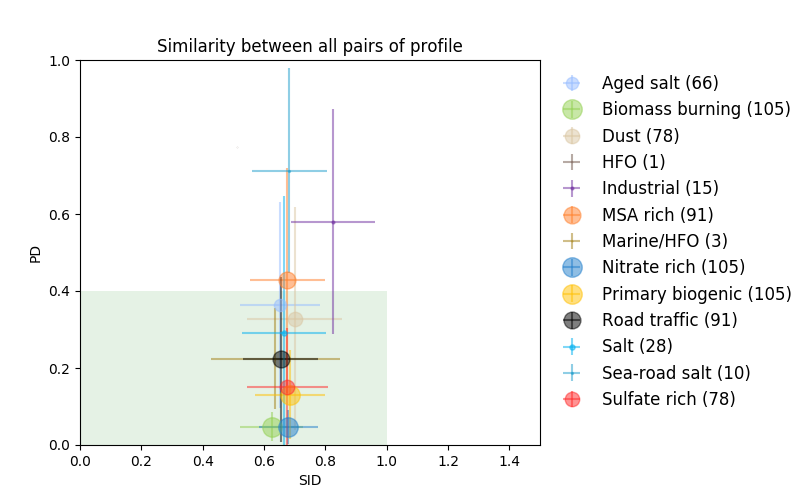
\includegraphics[width=0.8\linewidth]{figures/fig2}
    \caption{
        Similarity profile in the PD-SID space for all the pairs of PMF profile
        identified at all sites (see text for explanation). The mean (dot) and
        standard deviation (lines) are reported in the figure. The values in
        parenthesis indicate the number of pairs of profile considered: with $\binom{N}{2}$
        the number of site where the profile is identified.
    }%
    \label{fig:fig2}
\end{figure*}

To assess if PMF factors identically named are indeed similar in terms
of geochemistry, we reported similarity metrics (PD: Pearson distance
and SID: standardized identity distance defined in~\citep{pernigottiDeltaSA2018}) in
Figure~\ref{fig:fig2} for
all the identified profiles. The figure reports the mean and standard
deviation of the PD and SID for all possible pairs of profile but the
details for each given pair of profile may be found in the website.
According to~\citet{pernigottiDeltaSA2018}, two profiles are considered
similar if their PD and SID fall down the green rectangle delineating
the area with PD\textless0.4 and SID\textless1. We do observe a good
similarity (i.e. PD\textless0.4 and SID\textless1) for the main sources
of PM, namely biomass burning, nitrate-rich, primary biogenic, road
traffic, sulfate-rich. The dust, aged salt and MSA rich are often
identified and present acceptable SID, but do present important value
for the PD metric. As the PD is sensitive to ``extreme points'' that can
strongly affect the pearson correlation, this translates in our case
into the species contributing most to the PM mass (mainly OC and EC).
Then these profiles show differences in concentrations mainly for OC and
EC. The MSA-rich is found to be the most variable factor and a detail
analysis of the chemistry profile (see the website) indicates a lot of
differences for the concentration of EC but also
NO\textsubscript{3}\textsuperscript{-} and
NH\textsubscript{4}\textsuperscript{+} from site to site, where some
sites present contribution of theses species to the total PM mass
whereas other don't. Since it includes secondary organic species, its
variability may be explained by different formation or evolution
pathways (humidity, temperature, solar irradiation, etc.). We also point
out that the industrial source has a very diverse chemistry since it
gathers different local industrial processes. Nevertheless, the
geochemical stability of the majority of PMF factors on a regional scale
seems to us sufficient to consider that these emission sources have a
similar chemistry throughout France.

It is also interesting to note that the species contributing to
oxidizing potential have low concentration variability in the source
profiles emitting them. Indeed, previous studies pointed out the role of
transition metals in the OP of
PM~\citep{calasComparison2018,vermaOrganic2015,borlazaOxidative2018}.
In our source-apportionment, most of the copper in apportioned
by the road traffic source, which is then suspected to play a key role
in the observed OP\textsuperscript{DTT} and moreover to the
OP\textsuperscript{AA} value since the copper (Cu) is apportioned
between 34 \% to 54 \% (first and third quantile) by the road traffic
factor, with a concentration ranging from 1.7~ to 3.1~ of PM from this
source. We also note that the concentration uncertainties of Cu into the
road traffic is rather low (see website) as well as the concentration
variation across sites, suggesting that the intrinsic OP of this source
may be similar at the regional scale. Also, the levoglucosan, which
shows strong correlation to the OP\textsuperscript{DTT} and
OP\textsuperscript{AA}, is quasi-exclusively apportioned by the
biomass-burning source. Moreover, a lot of OC is contributing to the PM
of this factor and some metals (notably the copper) are apportioned by
this factor (10 \% of the total copper). The biomass burning is then
also strongly suspected to contribute to both OP in wintertime.

\subsection{OP seasonality}%
\label{op-seasonality}

The 15 time-series for both the OPDTT and OPAA at each site are
presented in SI and the website. A monthly aggregated view is given in
Figure~\ref{fig:fig3}, for both the
OP\textsubscript{v}\textsuperscript{DTT} and
OP\textsubscript{v}\textsuperscript{AA}. It is noted that the dataset
covers complete seasonality and is, in this sense, representative of a
regional climatology of the OP since it includes different sources with
different seasonal activities. Similar to the previous work
of~\citet{calasComparison2018,calasSeasonal2019}, extended by new yearly time-series, we observed a
seasonality of both the OP\textsubscript{v}\textsuperscript{DTT} and
OP\textsubscript{v}\textsuperscript{AA}, with higher values of OP during
the cold months compared to the warm months. We also note that during
the winter, the statistical distribution of OP values does not follow a
normal distribution and significant variability is observed. Notably,
and as shown in SI XX and already pointed out in~\citet{calasSeasonal2019},
the alpine sites present stronger seasonality compare to the others
(GRE-fr, GRE-cb, VIF, CHAM, MNZ, PAS). Also, some sites do not present
this seasonality, notably the traffic sites (RBX and STG-cle), the urban
traffic (NIC) or the industrial one (PdB). This seasonality could be
explained by the source of biomass combustion, which also exhibits this
type of seasonality, especially in the Alpine valleys, being the major
source of PM in these regions in winter. Also, as presented in the SI XX
and in~\citet{calasSeasonal2019}, some rapid variation of the
OP\textsuperscript{DTT} and OP\textsuperscript{AA} are observed, with
drastic increase or decrease within the frame of few days, similarly to
the PM10 mass, suspected to be linked with atmospheric circulation and
vertical mixing of the boundary layer, notably due to inversion layer
that traps the pollutants in the valley.


\begin{figure*}[ht]
    \centering
    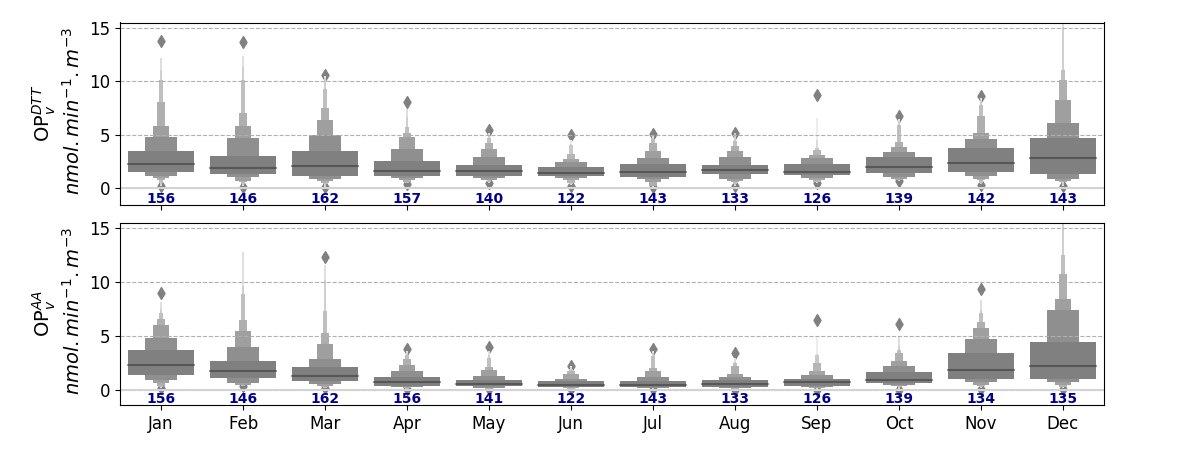
\includegraphics[width=1.0\linewidth]{figures/fig3}
    \caption{
    Boxenplot of OPvDTT and OPvAA seasonal value. The numbers in the x-axis
    indicate the number of observation. Each box represent one decile and the
    black line indicates the median of the distribution. Some values greater
    than 15.5 \uOPv are not displayed for graphical purpose. 
    }%
    \label{fig:fig3}
\end{figure*}

\subsection{Correlation OP -- sources}%
\label{correlation-op-sources}

This study focuses on the main drivers of OP at the regional scale. For
this reason, we decided to include in the main discussion only the PMF
factor identified at least two-thirds of the sites (i.e. 10 out of 15
sites), namely the aged salt, biomass burning, dust, MSA rich,
nitrate-rich, primary biogenic, primary road traffic and sulfate-rich
sources. The other local sources barely contributed to the total PM mass
and important uncertainties were often attached to them. The only
notable exception is the HFO profile identified at some coastal sites,
discussed hereafter in it's own section. We invite the reader to explore
the website to have the full view of the results.

In order to have a first estimate of the sources that can be associated
with the OP, the Spearman correlation between the source mass
apportionment from the PMF and the measured
OP\textsubscript{v}\textsuperscript{DTT} and
OP\textsubscript{v}\textsuperscript{AA} are presented in
Figure~\ref{fig:fig4}. This figure takes
into account all samples from all sites. First of all, the two OP shows
good correlation but do not carry the exact same signal
(r\textsubscript{OP DTT-OPAA}=0.61). Secondly, the only source that
strongly correlates to one OP (r\textgreater0.6) is the biomass burning
to the OP\textsubscript{v}\textsuperscript{AA}. Some mild correlation
(0.3\textless{} r\textless0.6) are found for the
OP\textsubscript{v}\textsuperscript{DTT} vs. road traffic, biomass
burning, nitrate-rich and dust and for the
OP\textsubscript{v}\textsuperscript{AA} vs. nitrate rich and road
traffic. This result is in line with previous study, either with the
source correlation~\citep{weberApportionment2018} or with the proxy of sources
(namely, levoglucosan for biomass burning and EC, iron, copper or PAH
for road
traffic)~\citep{calasComparison2018,calasSeasonal2019,charrierDithiothreitol2012,choRedox2005,huRedox2008,janssenAssociations2015,kunzliComparison2006,ntziachristosRelationship2007,pietrograndeChemical2018,vermaRedox2009,vermaReactive2014,borlazaOxidative2018}.
However, the nitrate rich source, mildly correlated
to both OP, doesn't present any atmospheric compound that are known to
be redox-active (to our knowledge). This correlation may then not
reflect any causality and the multilinear regression should disentangle
possible co-variation of the nitrate-rich source and other redox-active
one.

\begin{figure*}[ht]
    \centering
    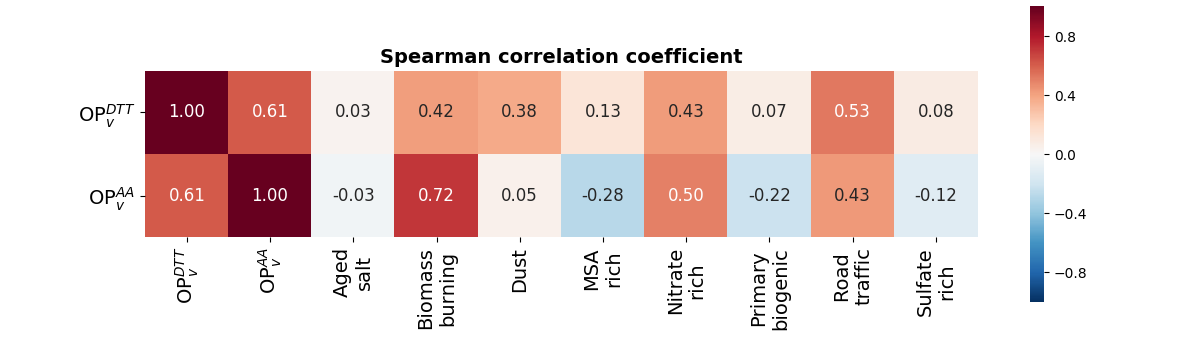
\includegraphics[width=1.0\linewidth]{figures/fig4}
    \caption{
        Spearman correlation coefficient between the OPvDTT and the OPvAA to the 8 PM
        sources identified at at least two third of the sites. All sites are grouped
        together in this figure, taking into account the whole time-series of measurement
        (number of observation days: Aged salt 1430; Biomass burning 1700, Dust 1489, MSA
        rich 1595, Nitrate rich 1700, Primary biogenic 1700, Road traffic 1587, Sulfate
        rich 1524).
    }%
    \label{fig:fig4}
\end{figure*}


\subsection{Accuracy of the MLR model}%
\label{accuracy-of-the-mlr-model}

The MLR statistical validation was carried out by a residual analysis
between the OP observed and the OP reconstructed by the model. For this
evaluation, the intrinsic OP of the sources was set to the mean of the
500 bootstrap values. Table~\ref{tab:tab2}
presents the fitted line between the modeled and observed
OP\textsubscript{v}\textsuperscript{DTT} and
OP\textsubscript{v}\textsuperscript{AA} together with the Pearson
correlation coefficient. Details and individual scatter plot are given
the SI XX. All but two sites present a very good correlation between
observed and reconstructed OP (r²\textgreater0.7) and a regression line
close to unity. We note that two models (STG-cle for AA and VIF for DTT)
present a clear lower correlation (r²=0.46 and 0.49, respectively)
together with the fitted line the farthest than the y=x line. However,
an in-depth analysis highlights that such a correlation is driven by few
days of observation on this regression (see SI XX). We therefore
consider our models valid for the rest of this study and each intrinsic
OP (i.e. coefficient of the regression) may be explored individually to
geochemically explain the observed OP.

\subsection{Limit of the linear model}%
\label{limit-of-the-linear-model}

Despite our models being able to reproduce most of the observations, we
can also see in figure SI XX that even if the MLR produces normally
distributed residuals (observation minus model), it also tends to
underestimate the highest values and the residuals are often
heteroscedastics (i.e. the higher values, the higher the uncertainties).
Then, the underlying hypothesis of linearity between endogenous
variables (source PM concentration) and exogenous variables (OP) may be
deemed invalid. The reader should keep in mind that non-linear processes
are strongly suspected for the source-apportionment of OP, as already
noted by~\citet{calasComparison2018} or~\citet{charrierBias2016}. As a result,
future developments on OP apportionment models should focus on this
suspected non-linearity, either with co-variations terms or even
non-linear model such as neural-network for instance.

\begin{table}[ht]
    \centering
    \caption{
    Observed vs reconstructed OP equation and Pearson correlation, taking the mean value
    of the 500 bootstraps, for all the sites.
    }
    \label{tab:tab2}
    \begin{tabular}{lll}
\tophline
    & \textbf{DTTv} & \textbf{AAv}\\
\middlehline
MRS-5av      & 0.77x+0.60 r²=0.72 & 0.69x+0.10 r²=0.72\\
PdB          & 0.87x+0.24 r²=0.84 & 0.91x+0.07 r²=0.87\\
AIX          & 0.91x+0.18 r²=0.82 & 1.01x+0.04 r²=0.92\\
NIC          & 0.76x+0.52 r²=0.79 & 0.88x+0.12 r²=0.83\\
TAL          & 0.76x+0.34 r²=0.77 & 0.83x+0.07 r²=0.86\\
NGT          & 0.81x+0.43 r²=0.75 & 0.97x+0.05 r²=0.87\\
GRE-fr\_2013 & 0.97x-0.14 r²=0.79 & 0.69x+0.20 r²=0.79\\
GRE-fr\_2017 & 0.77x+0.20 r²=0.81 & 1.02x+0.01 r²=0.94\\
GRE-cb       & 0.70x+0.35 r²=0.72 & 0.81x+0.20 r²=0.86\\
VIF          & 0.62x+0.47 r²=0.49 & 0.78x+0.20 r²=0.93\\
CHAM         & 0.87x+0.21 r²=0.90 & 0.85x+0.14 r²=0.93\\
MNZ          & 0.87x+0.19 r²=0.95 & 0.90x-0.01 r²=0.96\\
PAS          & 0.76x+0.72 r²=0.90 & 0.96x-0.06 r²=0.82\\
RBX          & 0.75x+0.49 r²=0.72 & 0.86x+0.31 r²=0.75\\
STG-cle      & 0.75x+0.57 r²=0.73 & 0.55x+0.64 r²=0.46\\
\bottomhline
    \end{tabular}
\end{table}

\subsection{Intrinsic OP per sources}%
\label{intrinsic-op-per-sources}

Even if the models reproduce the observations correctly, this does not
guarantee that the geochemical meaning extracted is the same for each of
the models, i.e. the intrinsic OP of the sources may completely differ
from site to site. The question is then to identify if a given source
contributes similarly to the OP at all sites. In other words, does all
model extract any geochemical general information relative to the OP?
Figure~\ref{fig:fig5} presents the intrinsic OP\textsuperscript{DTT} \textbf{A)} and
OP\textsuperscript{AA} \textbf{B)} for the selected subset of sources.
The values of all the N bootstraps for all the n stations where the
sources were identified (i.e. between \(500 \times 15 = 7500\) and
\(500 \times 10 = 5000\) values) are represented by the boxenplot to
display the value distribution, together with the mean and standard
deviation in white dots and lines, respectively. The exact values of
mean and standard deviation are also reported in
Table~\ref{tab:tab3} and details per
station for all sources are given in Table SI4.

\begin{figure*}[ht]
    \centering
    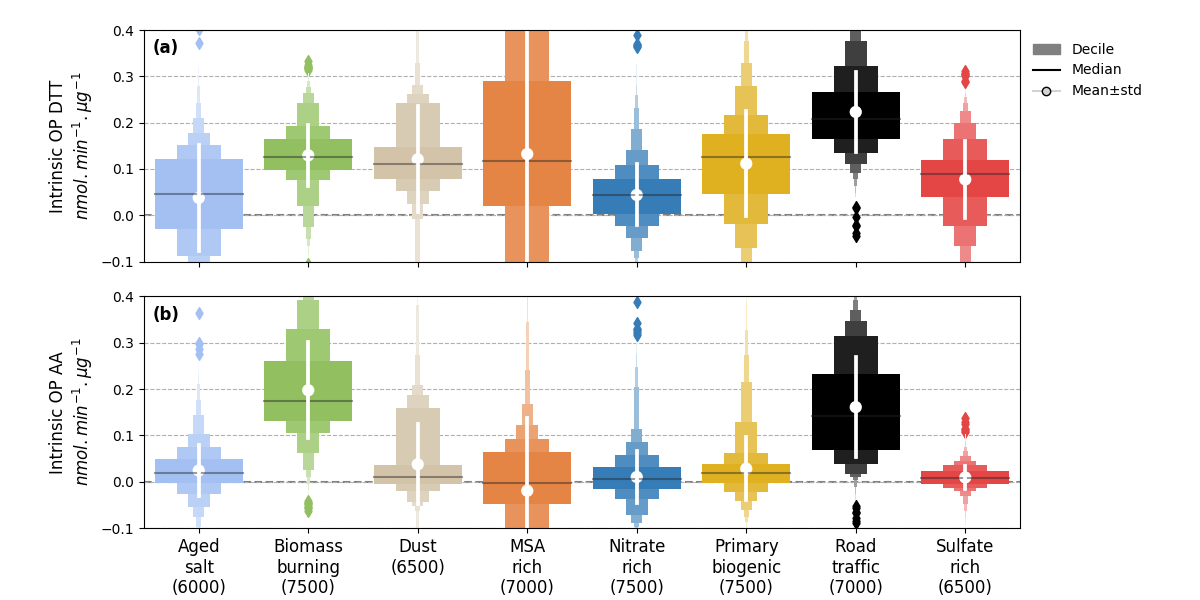
\includegraphics[width=1.0\linewidth]{figures/fig5}
    \caption{
        Intrinsic OP A) DTT and B) AA for the sources identified at at least two third of
        the site (i.e. 10 sites). The graphic displays the $n \times N$ intrinsic OP in
        parenthesis (with $n$ the number of site where the source was identified and
        $N=500$ bootstraps) and their statistical distribution via boxenplot: each box
        delimit a decile. The mean and standard deviation are also given in white dots and
        lines, respectively.
    }%
    \label{fig:fig5}
\end{figure*}

First of all, the mean values of the intrinsic OP are almost always
found positive when considering the whole dataset. The only case where a
small negative mean intrinsic OP found is for the MSA rich factor for
the AA assay (-0.018(152)), but strong variance is attached to this
result. It then confirms, if still needed, that airborne particles are
an oxidant material.

We also observe a net distinction of the intrinsic OP for the different
sources of PM, with intrinsic OP ranging from 0.044(64) to 0.223(85) for
the DTT and -0.018(152) to 0.197(104) for the AA. We confirm the
previous studies that also found different reactivity (or intrinsic OP)
for different sources based on RM
techniques~\citep{ayresEvaluating2008,batesReactive2015,cesariSource2019,costabileEvidence2019,fangOxidative2016,paraskevopoulouYearlong2019,perronePM22019,vermaReactive2014,weberApportionment2018,zhouPredominance2019}.
Notably, the road traffic
source is the most reactive source toward the OP\textsuperscript{DTT},
with a value of 0.223(85) which is almost twice the value of the other
group of reactive source, namely 0.132(410), 0.129(65), 0.121(114) and
0.112(113) for the MSA rich, biomass burning, dust and primary biogenic
sources, respectively. Interestingly, the nitrate-rich factor is the
second most correlated to the OP\textsubscript{v}\textsuperscript{DTT}
but is the one associated with the lowest intrinsic
OP\textsuperscript{DTT} (0.044(65)). Concerning the intrinsic
OP\textsuperscript{AA}, less sources present redox activity. Notably,
only the biomass burning and road traffic present an intrinsic OP easily
distinguishable from 0, with respect to the uncertainties with intrinsic
OP\textsuperscript{AA} of 0.197(103) and 0.161(108), respectively.
Overall, it appears that the intrinsic OP of the different sources
(expect the MSA-rich) are similar at a regional level, paving the road
to the implementation of OP in CTM.

Overall, the OP\textsuperscript{DTT} is more balanced than the
OP\textsuperscript{AA} as already pointed by~\citet{fangOxidative2016}
and~\citet{weberApportionment2018} and seems to target all the sources containing
either metals and organic species but is not sensitive to ammonium
nitrate source. OP\textsuperscript{AA} mainly target biomass burning and
primary road traffic factor, as already pointed out in previous
studies~\citep[][and references therin]{batesReview2019}. We then confirm what
previous studies found either by direct OP measurement at the source or
by source -apportionment. It is however hard to directly compare the
absolute value of our result to the literature since all protocols vary
from one group to another. The coefficient of variation (CV, standard
deviation over mean) of the intrinsic OP are the lowest for the
\textbf{biomass burning} and primary \textbf{road traffic} for the DTT
assay with values of 0.5 and 0.38, respectively, as well as for the AA
assay with value of 0.52 and 0.67, respectively. The variability of the
biomass burning intrinsic OP is more site dependent, with a low
uncertainty at any given site, but with slightly different intrinsic OP
between sites. It then suggests that the variability is not linked to
uncertainties of the model but from local variation of the chemistry of
this profile. However, the biomass burning is the most geochemically
stable profile in our dataset, with a PD \textless{} 0.1 and SID
\textless{} 0.7. Hence, the variability should come from species not
measured in our dataset. Namely, no PAH, oxy-PAH, OH-PAH nor quinone are
measured, although they are known to contribute to the
OP~\citep{charrierDithiothreitol2012} and have short live time and being heavily influenced
by the climatic condition~\citep{mierschImpact2019}. The road traffic
chemical profile is also similar at all sites (with the exception of RBX
and VIF where mixing effects are observed) with our given set of
species. Moreover, the uncertainty of the road traffic intrinsic OP at
each site lies in the uncertainties of the other sites. Hence, the low
variability for the OP\textsuperscript{DTT} indicates that the observed
species, similar at each sites, are the one that influence
OP\textsuperscript{DTT}. However, for the OP\textsuperscript{AA} the
variability is higher with some important difference from site to site,
without clear distinction by typology or groups of sites. Then, some
species that are not measured here may influence the
OP\textsuperscript{AA}, but not the OP\textsuperscript{DTT}.

The inorganic factor (\textbf{sulfate-rich} and \textbf{nitrate-rich})
presents a high CV. However, the CV may not be an accurate measure for
some sources with near 0 mean intrinsic OP. The standard deviation is
similar to the one of the biomass burning and road traffic for the OP
DTT, and are among the lowest variability for the OP\textsuperscript{AA}
(see table REF). The two inorganic factor are also very similar at each
site in term of chemical composition, as presented in the SID-PD space
in Figure~\ref{fig:fig2}.

The \textbf{dust} source presents an important variability when taking
into account the whole sites, but a deeper analysis shows 2 groups of
sites: AIX-RBX-VIF and the others. The first group presents high
intrinsic OP for both assays, whereas the others display half
(OP\textsuperscript{DTT}) or almost null (OP\textsuperscript{AA})
intrinsic OP (see table XXX). Then, the first conclusion is that 80 \%
of the sites agree on a common intrinsic OP for the dust source. The
high variability for VIF may be explained by different chemistry.
Indeed, the dust factor at VIF highly differs from the other dust
factors with a PD \textgreater{} 0.75 when compared to the other sites
(see SUP INFO). We don't have clear hypothesis yet for the two others
sites.

Despite the different PMF (and so number of sources) solution at each
site and the different OP signal, the rather low variability of the
intrinsic OP for a given source suggests that a given source of PM
behave similarly at each site with regards to the OP. It then supports
the idea that, at the national scale, the sources described above have a
determined and stable intrinsic OP. This result achieved the very first
requirement before a potential implementation of the OP in deterministic
chemistry transport model (CTM).

\subsubsection{Variability of the biogenic and organic sources}%
\label{variability-of-the-biogenic-and-organic-sources}

High variability is found for the \textbf{MSA rich} source with high
variability between sites but also at a given site, with a CV of 3.1 and
7.8 for the DTT and AA assay, respectively.

The secondary organic source appears to be the most variable source in
term of intrinsic OP, notably for the DTT assay. The MSA rich factor is
the one among the 8 major sources of PM that contributes the less to the
total PM mass and the PMF bootstrap result presents important
variability for the PM\textsubscript{10} apportioned by this source. In
our study, the secondary organic factor (SOA) is mainly traced by the
MSA, but its remaining composition is yet unknown. This PMF factor is
still not yet fully understood and few studies reported it so far. As a
result, we don't know for instance the loading of HULIS, quinone or
isoprene derived compounds in this factor, nor the amount of aging this
factor encountered at each site. Such unknown is reflected in the MSA
rich factor being the less similar factor between sites (see previous
similarity assessment section). Such uncertainties on the chemistry of
this factor may explain the diversity if intrinsic OP observed. Indeed,
it has been shown that SOA species may contribute to the
OP\textsuperscript{DTT} in the early stage of aging~\citep{mcwhinneyNaphthalene2013}
or to the OP\textsuperscript{DCFH}~\citep{zhouParticlebound2018}, but due to
aging processes and photochemical degradation, aged SOA species may
contribute to a lesser extent to it~\citep{jiangDynamic2018,wangRelationship2017}.
But~\citet{vermaRedox2009,vermaFractionating2015} pointed that aging of SOA may
increase the OP. Moreover,~\citet{tuetChemical2019} shown that humidity and
seed particles have also an effect on SOA OP\textsuperscript{DTT}. Since
all these parameters vary in our study, it may explain the diversity of
chemistry and thus intrinsic OP\textsuperscript{DTT} we observed for
SOA. To a lesser extent, this variability is also found for the AA
assay, suggesting that the same phenomena affects the SOA
OP\textsuperscript{AA}. The sulfate-rich factor is also suspected to
account for some SOA since OC are present in non-negligible amounts.
Then, the variability of the sulfate-rich, and similarly for the
\textbf{aged sea-salt}, intrinsic OP may be explained by the same
phenomena.

Also the \textbf{primary biogenic source}, mainly traced by polyols,
presents some variability for the OP\textsuperscript{DTT}. \citet{samakeUnexpected2017}
highlighted that spore or bacteria does contribute to the
OP\textsuperscript{DTT} and OPAA activity, even if the microbial cells
are dead. However, the authors also present the inhibition of the DTT
loss rate in presence of metals and 1,4-naphtoquinone or Cu. Since both
results are observed, depending on which microbiota are living on the
sampled PM, intrinsic OP\textsuperscript{DTT} may be enhanced or
decreased. The variability of intrinsic OP\textsuperscript{DTT} observed
in Figure 5 may then reflect the local different microbiology living in
the PM or covariation of the primary biogenic source with another metal
or 1,4-naphtoquinone rich source for instance. Also,~\citet{samakePolyols2019}
pointed that some secondary species may be incorporated in this
factor at some site, making it a mix of primary biogenic and SOA,
another hypothesis is the ``aging'' of this factor. It is then possible
that the SOA mixed in the primary biogenic may influence the intrinsic
OP in different way, similarly to the MSA rich factor.

\begin{sidewaystable*}[ht]
    \caption{
        Intrinsic OP\textsuperscript{DTT} and AA for the 8 main sources of PM. The value
        are the mean and standard deviation of the 500 bootstraps. Unit are in
        \uOPm.
    }
    \label{tab:tab3}
    \begin{tabular}{llllllllll}
\tophline
\textbf{OP type} & \textbf{station}             & \textbf{Aged salt} & \textbf{Biomass burning} & \textbf{Dust} & \textbf{MSA rich} & \textbf{Nitrate rich} & \textbf{Primary biogenic} & \textbf{Road traffic} & \textbf{Sulfate rich}\\
\middlehline
\textbf{DTT}     & \textbf{All stations and BS} & 0.038(113)  & 0.129(65)  & 0.121(114) & 0.132(410)  & 0.044(65)  & 0.112(113)  & 0.223(85)  & 0.077(82)\\
                 & AIX                          & -0.134(55)  & 0.107(28)  & 0.224(58)  & 0.051(63)   & 0.015(70)  & 0.072(72)   & 0.200(74)  & -\\
                 & CHAM                         & -           & 0.092(6)   & 0.087(18)  & 0.240(49)   & 0.065(28)  & 0.131(17)   & 0.406(60)  & 0.082(17)\\
                 & GRE-cb                       & 0.018(46)   & 0.105(26)  & 0.122(21)  & 0.779(210)  & 0.053(21)  & 0.282(68)   & 0.163(42)  & -0.017(33)\\
                 & GRE-fr\_2013                 & 0.181(69)   & 0.261(22)  & 0.131(32)  & 0.080(136)  & -0.021(60) & 0.165(47)   & 0.206(33)  & 0.186(30)\\
                 & GRE-fr\_2017                 & -0.083(163) & 0.102(47)  & 0.094(39)  & -0.173(323) & 0.008(18)  & 0.237(125)  & 0.183(38)  & 0.054(35)\\
                 & MRS-5av                      & 0.110(44)   & 0.114(68)  & 0.025(22)  & 0.168(224)  & 0.088(102) & -0.046(90)  & 0.243(53)  & 0.025(35)\\
                 & MNZ                          & -           & 0.116(5)   & 0.069(15)  & 0.095(31)   & 0.053(7)   & 0.071(9)    & 0.253(18)  & 0.086(7)\\
                 & NIC                          & 0.120(26)   & 0.117(13)  & 0.110(27)  & -           & 0.081(46)  & 0.004(48)   & 0.279(84)  & 0.082(24)\\
                 & NGT                          & 0.116(43)   & 0.191(35)  & -          & 0.533(298)  & 0.023(35)  & -0.038(114) & 0.159(35)  & 0.198(46)\\
                 & PAS                          & -           & 0.129(11)  & 0.109(15)  & 0.161(75)   & 0.161(55)  & 0.186(31)   & 0.256(44)  & 0.114(21)\\
                 & PdB                          & 0.032(32)   & 0.179(14)  & 0.140(19)  & 0.123(80)   & 0.017(22)  & 0.161(26)   & -          & 0.098(35)\\
                 & RBX                          & -0.006(50)  & -0.018(43) & 0.251(16)  & -0.096(72)  & 0.066(9)   & 0.004(42)   & 0.189(28)  & -0.106(46)\\
                 & STG-cle                      & 0.137(37)   & 0.155(17)  & -          & 0.370(71)   & 0.084(18)  & 0.154(35)   & 0.197(18)  & 0.098(21)\\
                 & TAL                          & -0.044(30)  & 0.147(19)  & 0.103(21)  & 0.063(43)   & -0.036(32) & 0.142(45)   & 0.272(96)  & -\\
                 & VIF                          & 0.004(68)   & 0.144(28)  & 0.105(344) & -0.540(870) & 0.002(19)  & 0.148(38)   & 0.116(32)  & 0.106(25)\\
\textbf{AA}      & \textbf{All stations and BS} & 0.024(54)   & 0.197(103) & 0.037(86)  & -0.020(156) & 0.010(56)  & 0.028(67)   & 0.161(108) & 0.009(24)\\
                 & AIX                          & -0.049(46)  & 0.194(18)  & 0.157(27)  & 0.051(58)   & 0.118(82)  & 0.030(68)   & 0.221(68)  & -\\
                 & CHAM                         & -           & 0.174(12)  & -0.048(15) & 0.001(37)   & -0.032(39) & 0.025(15)   & 0.297(43)  & -0.011(8)\\
                 & GRE-cb                       & -0.007(27)  & 0.169(36)  & -0.015(16) & -0.169(103) & 0.030(12)  & 0.015(38)   & 0.196(24)  & 0.029(10)\\
                 & GRE-fr\_2013                 & 0.037(19)   & 0.183(11)  & 0.012(11)  & -0.036(32)  & -0.004(14) & 0.032(14)   & 0.129(9)   & 0.002(13)\\
                 & GRE-fr\_2017                 & 0.103(83)   & 0.368(26)  & 0.017(8)   & -0.016(100) & -0.036(17) & -0.010(36)  & 0.182(20)  & 0.042(11)\\
                 & MRS-5av                      & 0.016(7)    & 0.101(12)  & 0.004(7)   & -0.029(34)  & 0.004(9)   & 0.001(18)   & 0.023(15)  & 0.001(6)\\
                 & MNZ                          & -           & 0.266(12)  & 0.006(11)  & 0.082(16)   & -0.084(30) & 0.027(9)    & 0.154(22)  & 0.014(9)\\
                 & NIC                          & 0.034(22)   & 0.112(11)  & -0.001(16) & -           & -0.018(17) & -0.034(28)  & 0.354(47)  & 0.013(10)\\
                 & NGT                          & 0.069(31)   & 0.428(60)  & -          & -0.078(234) & 0.063(35)  & 0.225(95)   & 0.074(46)  & -0.016(38)\\
                 & PAS                          & -           & 0.161(13)  & -0.002(7)  & -0.013(35)  & 0.040(58)  & 0.007(16)   & 0.047(23)  & -0.003(15)\\
                 & PdB                          & 0.011(14)   & 0.138(7)   & 0.034(8)   & -0.003(26)  & -0.011(15) & 0.035(11)   & -          & 0.006(8)\\
                 & RBX                          & 0.069(26)   & 0.223(42)  & 0.167(23)  & 0.090(63)   & 0.019(12)  & 0.036(40)   & 0.317(39)  & 0.028(36)\\
                 & STG-cle                      & -0.023(30)  & 0.026(25)  & -          & 0.080(20)   & 0.044(12)  & 0.015(25)   & 0.128(17)  & -0.007(11)\\
                 & TAL                          & 0.008(17)   & 0.134(15)  & 0.006(9)   & -0.015(30)  & 0.004(10)  & 0.004(27)   & 0.081(51)  & -\\
                 & VIF                          & 0.021(41)   & 0.284(23)  & 0.150(181) & -0.221(385) & 0.015(20)  & 0.014(22)   & 0.052(15)  & 0.021(9)\\
\bottomhline
    \end{tabular}
\end{sidewaystable*}

\subsection{Contribution of the sources to the OP}%
\label{contribution-of-the-sources-to-the-op-1}

Since the intrinsic OP of the 8 sources may be considered as stable
(except the MSA-rich), we can estimate the sources contribution to the
OP, similarly to the sources contribution to the PM concentration. In
this part, we estimate the contribution of the sources to the OP and PM
concentration at each sites, then present an aggregated view of the
seasonal contribution in Figure~\ref{fig:fig6}, and the daily contribution in
Figure~\ref{fig:fig7} and~\ref{fig:fig8}, taking into account all the sites. Since our dataset included
an important proportion of alpine sites and given the fact that all
sites are urbanized, the extrapolation to the whole France or other
region should be done cautiously. Also, only the contributions of the 8
previously selected sources are reported here. The full results with
details per site are presented in the website mentioned above.

\subsubsection{Seasonality of the contribution}%
\label{seasonality-of-the-contribution}

\begin{figure*}[ht]
    \centering
    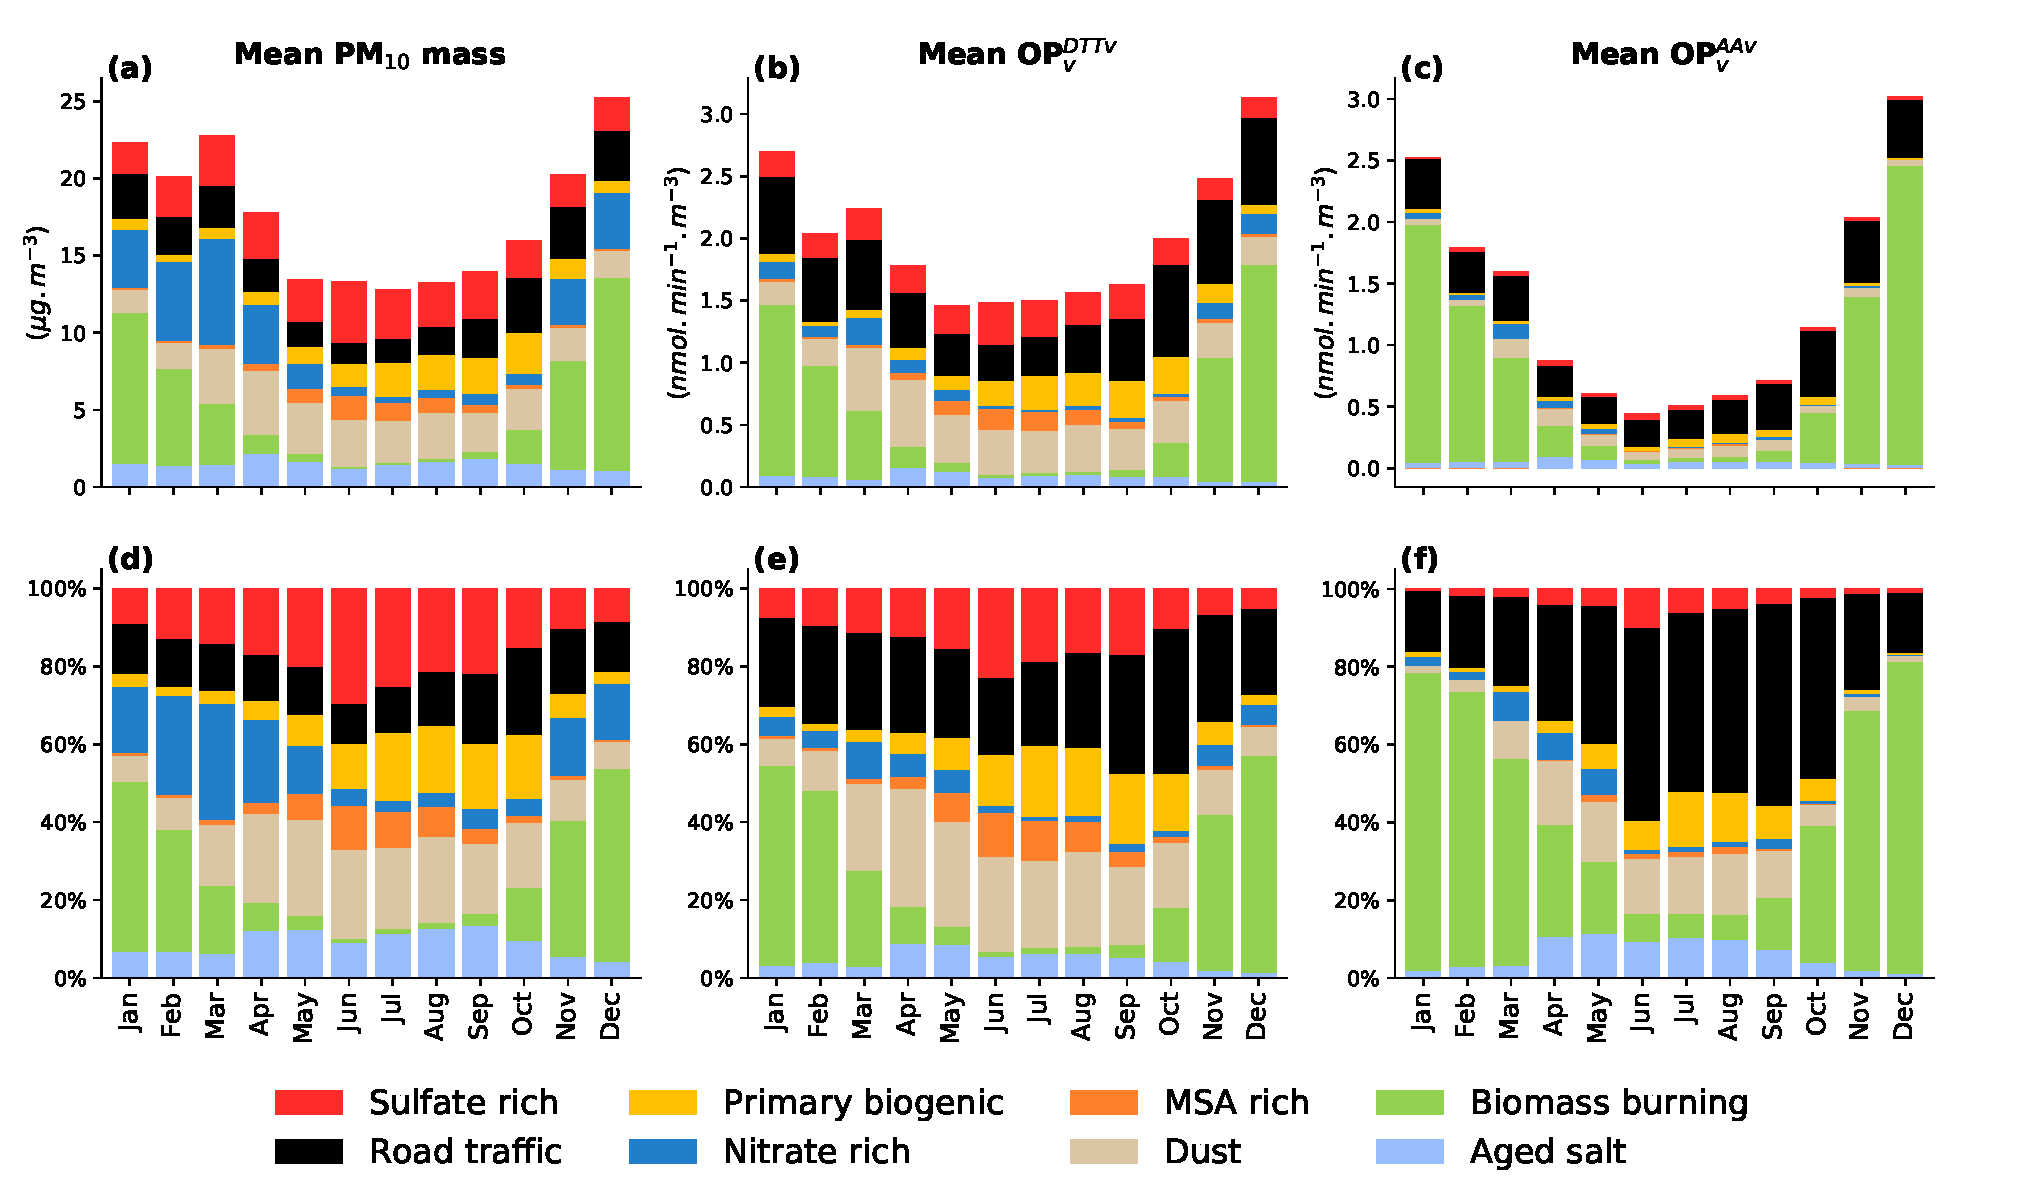
\includegraphics[width=1.0\linewidth]{figures/fig6}
    \caption{
    Mean monthly contribution of the main 8 sources to the \textbf{(a)} PM10 mass, \textbf{(b)}
    OPvDTT and \textbf{(c)} OPvAA taken into account each sources contribution of every
    sites; and there respective normalized contribution in \textbf{(d)} PM10 mass, \textbf{(e)}
    OPvDTT and \textbf{(f)} OPvAA (taking into account only these 8 sources). 
    }%
    \label{fig:fig6}
\end{figure*}

It is already known and well documented that PM\textsubscript{10} mass
concentration presents a seasonality, notably in alpine valley due to
the biomass burning source and meteorological effects. By construction,
the contribution to OPDTTv and OPAAv from each source is proportional to
the mass contribution of the source in question. However, the relative
importance of the contributions of the sources is altered by the fact
that they have different intrinsic OPs. The question, therefore, is what
are the sources of PM that contribute the most to the OP. The mean
monthly contribution of the 8 sources from all sites to the
PM\textsubscript{10} mass, OP\textsubscript{v}\textsuperscript{DTT} and
OP\textsubscript{v}\textsuperscript{AA} are presented in
Figure~\ref{fig:fig6} \textbf{(a)},
\textbf{(b)} and \textbf{(c)}, respectively.

As already shown by previous study in
France~\citep{favezTraitement2017,petitSources2019,srivastavaSpeciation2018a,wakedSource2014,weberComparison2019},
the seasonal mean contribution to the PM\textsubscript{10} mass
show the importance of the biomass burning source, followed by the
secondary inorganic (sulfate-rich and nitrate-rich), the dust and road
traffic. But as a direct consequence of the different intrinsic OP, we
do observe a redistribution of the relative importance of the sources.
Namely, the nitrate-rich source that may contribute to a significant
amount to the PM\textsubscript{10} mass, notably in spring, barely
contribute to the OP\textsubscript{v}\textsuperscript{DTT} nor to the
OP\textsubscript{v}\textsuperscript{AA}. Conversely, the road traffic
contributes to about 15 \% during summer to the mean
PM\textsubscript{10} mass but is more than 50 \% of the mean
OP\textsubscript{v}\textsuperscript{AA} in the same period of time
(Figure~\ref{fig:fig6} \textbf{(d)},
\textbf{(e)} and \textbf{(f)}). However, the biomass burning sources is
still a major contributor to both the
OP\textsubscript{v}\textsuperscript{DTT} and
OP\textsubscript{v}\textsuperscript{AA} during winter months. We note
that the primary biogenic source still contributes to the
OP\textsubscript{v}\textsuperscript{DTT} but to a lesser extent to the
OP\textsubscript{v}\textsuperscript{AA}. Also the dust source continues
to be an important contributor to the
OP\textsubscript{v}\textsuperscript{DTT} but not to the
OP\textsubscript{v}\textsuperscript{AA}. These results tend to confirm
what previous studies already found. With regard to the seasonality of
OP, regulations should target the biomass burning emission in order to
decrease the PM\textsubscript{10} OP during winter by a large amount,
but also the road traffic that contributes homogeneously to both OP all
around the year.

\subsubsection{Daily mean and median contribution}%
\label{daily-mean-and-median-contribution}

\begin{figure*}[ht]
    \centering
    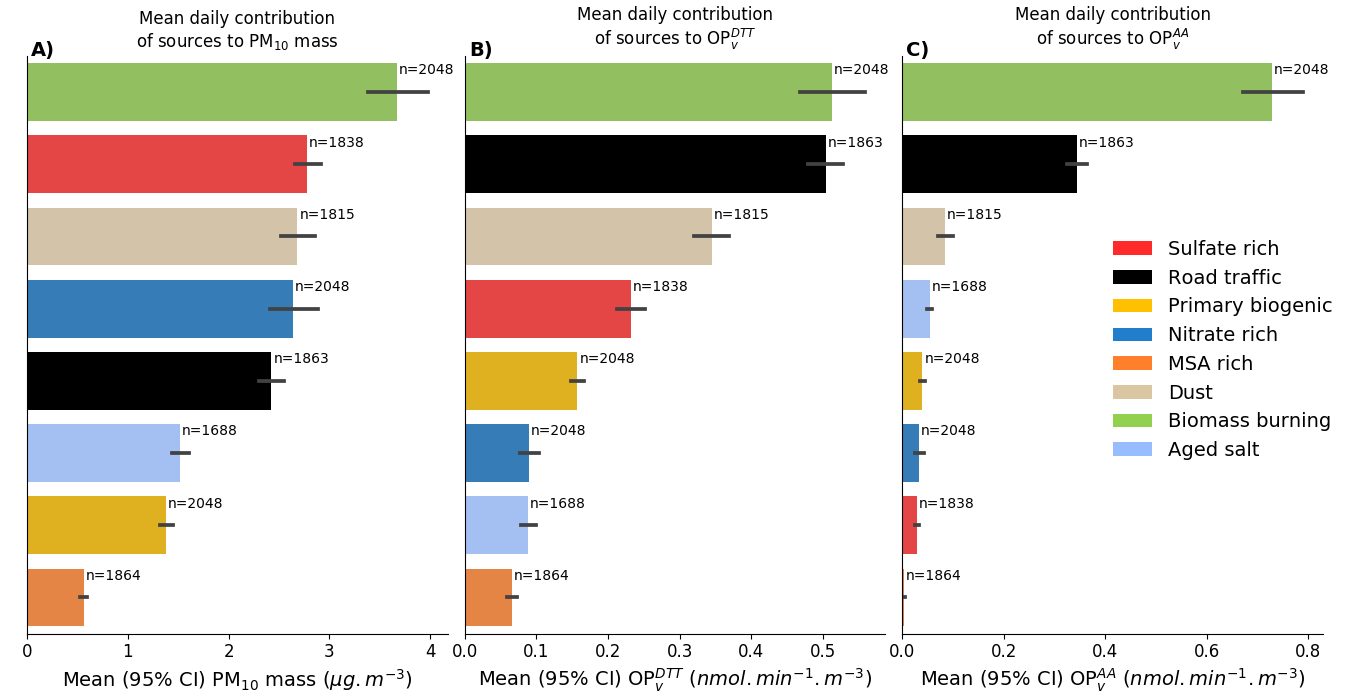
\includegraphics[width=1.0\linewidth]{figures/fig7}
    \caption{
    Averaged daily contribution of the sources to \textbf{(a)} the PM10 mass, \textbf{(b)} the
    OPvDTT and \textbf{(c)} the OPvAA. The bars represent the mean and the error bars the
    95 \% confidence interval of the mean.
    }%
    \label{fig:fig7}
\end{figure*}

\begin{figure*}[ht]
    \centering
    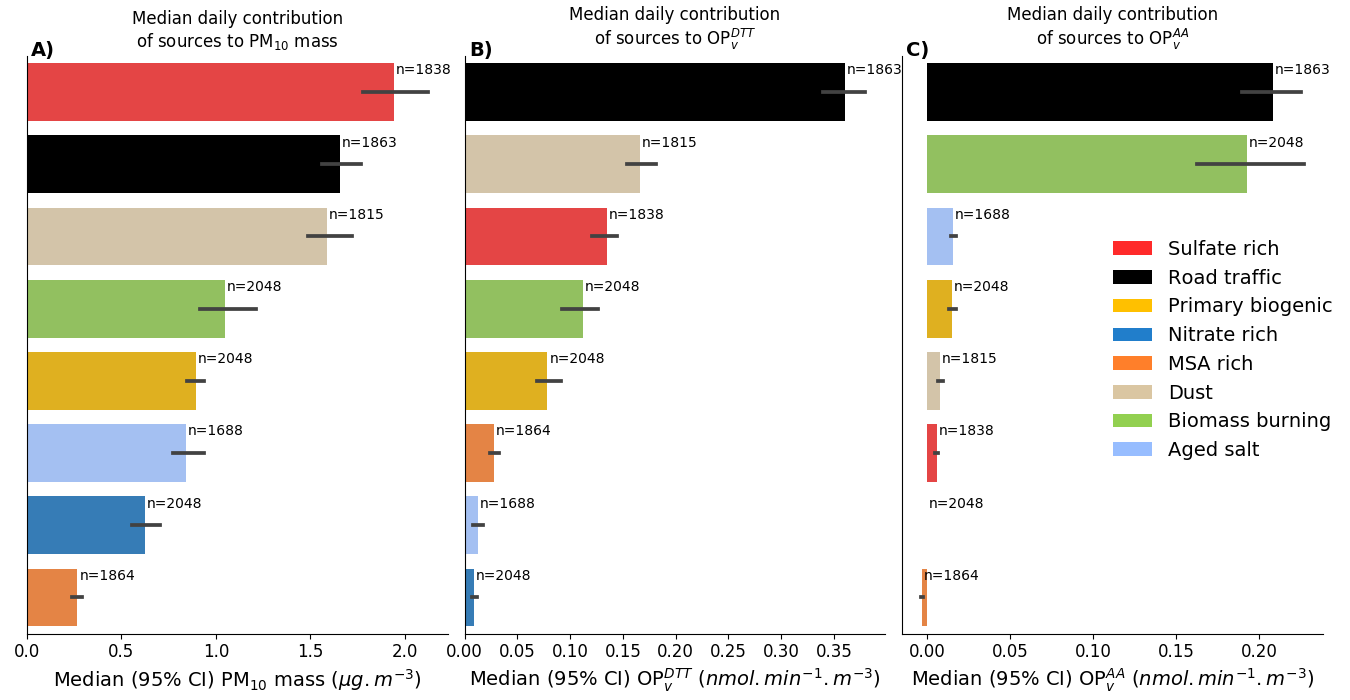
\includegraphics[width=1.0\linewidth]{figures/fig8}
    \caption{
        Median daily contribution of the sources to \textbf{(a)} the PM mass, \textbf{(b)} the
        OPvDTT and \textbf{(c)} the OPvAA. The bars represent the mean and the error bars
        the 95 \% confidence interval of the median. 
    }%
    \label{fig:fig8}
\end{figure*}

The seasonal mean contribution of the source may not take into account
the rapid day-to-day variability of the OP observed in SI XXX. Moreover,
most epidemiological studies average the yearly exposition to a ``daily
averaged'' or ``daily median'' exposure~\citep{worldhealthorganizationAmbient2016}.
In this part, we try to express the population exposition to the
sources to both the mass and OP metric on a daily basis.

The daily contribution is shown in Figure~\ref{fig:fig7} and Figure~\ref{fig:fig8}, for
the mean and median daily contribution, respectively. The results highly differ if
considering the mean or the median contribution, and the two statistical indicators do not
answer the same question. In particular, mean contribution is determined by the sum of
individual measurements making it highly sensitive to outliers. On the other hand, median
contribution is the middle value when the measurements in the actual dataset are arranged
in ascending order. The skewness of the distribution is not surprising as some high
PM\textsubscript{10} events (i.e., outliers in the dataset) were present in our
measurements. This is also specifically anticipated in alpine areas (XX out of 15 sites)
where the development of atmospheric inversions causing increased pollutant concentrations
are highly favorable.

Therefore, the mean contribution is more related to the question
``\emph{What Which sources contribute the most to the
PM\textsubscript{10} OP or mass?}'' whereas the median contribution
addresses the question ``\emph{What is the} \emph{chronic}
\emph{population exposure to the PM\textsubscript{10} OP or mass?}''.
Since there is strong seasonality, day-to-day variability and non-
normally distributed contribution of the source to the
PM\textsubscript{10} mass, notably for the biomass burning, we do
observe important differences when looking at the mean or median
contribution. Therefore, we decided to report both statistics in this
study. Here again, we want to remind the reader that our dataset
includes several alpine site strongly affected by the residential
biomass burning heating, then the result might not reflect the overall
regional exposure.

We do observe (Figure~\ref{fig:fig7}) a
redistribution of the daily \textbf{mean} contribution sources' rank
between the PM\textsubscript{10} mass,
OP\textsubscript{v}\textsuperscript{DTT} and
OP\textsubscript{v}\textsuperscript{AA} similarly to the monthly mean
contribution shown above. Since the biomass burning source is an
important contributor to the PM\textsubscript{10} mass, it contributes
also significantly to both OP and is ranked as the first contributor to
both OP\textsubscript{v}\textsuperscript{DTT} and
OP\textsubscript{v}\textsuperscript{AA} mean daily contribution (mean
0.51 and 0.72, respectively). The road traffic source contribution, due
to its highest intrinsic OP in both assays, has almost the same daily
mean contribution than the biomass burning for the
OP\textsubscript{v}\textsuperscript{DTT}, and is the second contributor
to the daily mean OP\textsubscript{v}\textsuperscript{AA}, with half the
contribution of the biomass burning (mean 0.50 and 0.34, respectively).
The other source barely not contribute to the
OP\textsubscript{v}\textsuperscript{AA} (\textless0.1 ). For the
OP\textsubscript{v}\textsuperscript{DTT}, the dust is the third
contributor (mean 0.34), followed by the sulfate rich and primary
biogenic (0.23 and 0.16 , respectively). The nitrate-rich, aged seasalt
and MSA-rich present a low contribution (mean \textless0.1), due either
to their low intrinsic OP or to their low contribution to the PM mass.

However, for the daily \textbf{median} contribution, due to the high
seasonality of the biomass burning source and the consistent
contribution throughout the year of the road traffic, sulfate-rich and
dust sources, the ranks of the sources is even more drastically
redistributed between all the considered metric
(Figure~\ref{fig:fig8}) A) mass, B)
OP\textsubscript{v}\textsuperscript{DTT} and C)
OP\textsubscript{v}\textsuperscript{AA}). Moreover, the absolute value
of the contribution is also lowered compare to the mean daily
contribution, due to low frequencies of highly loaded PM events. The
major source contributing to the
OP\textsubscript{v}\textsuperscript{DTT} is now the road traffic (median
0.36) and contributes more than twice as much as the second source,
namely the dust one (median 0.16 ), followed by the sulfate-rich (median
0.13 ) and then the biomass burning (median 0.11 ). For the
OP\textsubscript{v}\textsuperscript{AA}, the two dominant sources are
the road-traffic (median 0.29 ) and the biomass burning (median 0.19 ).
The others sources being negligible in front of them (aged seasalt 0.016
, primary biogenic 0.015 and the others contributes less than 0.01 ).

The high differences between the mean and median contribution has strong
implication for air quality policy. Indeed, as previously shown, the
biomass burning may contribute to more than 50 \% of the high OP during
winter, and even more for some days. However, such events do not
represent the daily exposure of the population. Even if the regulation
should target those events to prevent acute exposure, we should also
take into account the long term exposure to a lower but constant level
of pollutant. With this respect, the biomass burning source impact is
drastically lowered but the road traffic emission become a major
concern. Moreover, our dataset includes several site in alpine valley
that bias our result toward a more important contribution of the biomass
burning source compare to the actual urbanized French cities. Then, our
conclusion strongly supports that at the regional scale, the important
source to target in order to decrease the chronic exposure to PM
pollutant is the road traffic one. However, site specific typologies
(notably alpine valley, or ``hot spot'' with specific sources) may also
target other sources, notably the biomass burning source in alpine
valley, to prevent acute exposure of the population.

\subsection{Other PMF factors}%
\label{other-pmf-factors}

So far, we have focused on sources with regional impact. However, we
would like to discuss the case of 2 sources that are often controversial
for political decision-makers or inhabitants but are less representative
of the urban background of French cities.

\subsubsection{Heavy fuel oil}%
\label{heavy-fuel-oil}

Among the others sources, not present at at least 2 third of the site,
the Heavy fuel oil (HFO) identified at MRS-5av and PdB, present an
intrinsic OP\textsuperscript{DTT} of 0.51(14) and 0.21(4), respectively,
and an intrinsic OP\textsuperscript{AA} of 0.04(2) and 0.11(3),
respectively. The intrinsic OP\textsuperscript{DTT} is then in average
higher than the road traffic one, making the HFO the second contributor
of the daily mean and median source contribution at MRS-5av for the
OP\textsuperscript{DTT} contribution and the fourth one for the
OP\textsubscript{v}\textsuperscript{AA} contribution (see website
\url{http://getopstandop.u-ga.fr}). For PdB, an important contribution, but
lower than for MRS-5av is found, for both the DTT and AA. Although only
2 sites presented an HFO factor, it suggests that the PM originated from
this source may significantly contribute to the total OP around harbor
cities.

\subsubsection{Industrial}%
\label{industrial}

An industrial factor was identified at 6 sites. However, the
``industrial'' name for this factor cover a wide variety of chemistry,
as denoted in the similarity
Figure~\ref{fig:fig2}. They share a common
set of metal (Al, As, Cd, Mn, Mo, Pb, Rb, Zn), in different
concentration levels. Since we are not aware of any emission source
releasing these metals jointly into the atmosphere, we have named this
factor "Industrial", although the exact type of industry is not yet
known. This factor also barely contributes to the PM\textsubscript{10}
mass, with a mean concentration of around 1. The intrinsic
OP\textsuperscript{DTT} is high for GRE-cb and GRE-fr\_2017 (0.52(30)
and 0.37(27), respectively) as well as the intrinsic
OP\textsuperscript{AA} (0.82(29) and 0.61(17) , respectively), but is
close to 0 for the other sites and both OP. The high intrinsic OP seems
to indicate again the role of metals in the OP of PM, however since this
factor has strong uncertainties associated with the PMF results, and
then to the intrinsic OP, is hard to go into further conclusion at this
point.

\section{Limitations of the study}%
\label{limitations-of-the-study}

In this study, we focused on major sources and trends, hence limit our
study to some aspect. Notably the PMF standardized approach allows
common source identification at the national scale but may also
``polish'' some site specificity. Also, the choice to focus on the main
sources of PM and to discuss the aggregated results allows discussion on
some local specificity, notably potential local sources that contribute
to the OP (for instance HFO or industry).

One main limitation is also the use of linear regression tools whereas
it has been shown that OP does not respond linearly with mass. The
residual analysis seems to agree with this experimental finding since
the highest OP samples is underestimated by the MLR model. The addition
of co-variation term or even the use of non-linear regression may be the
next step to better explain the OP of the sources and provide more
accurate policy for air quality.

Moreover, if the intrinsic OP results from the MLR can be extrapolated
to any given site with similar regional background of the urbanized area
used in this study, the source' contributions extrapolation should be
taken cautiously since our dataset displays an over-representation of
the alpine sites with regard to the whole France.

\conclusions  %% \conclusions[modified heading if necessary]

To our knowledge, this study gathers the most important database of OP
samples with concomitant observations of chemistry analysis,
source-apportionment through PMF and the measure of two OP assays (DTT
and AA) for 15 yearly time series over France spanning between 2012 to
2016 for a total of \textgreater1700 samples.

\begin{itemize}
\item
  We demonstrate that source apportionment of OP through a ``simple''
  multi linear regression without any constraint on the coefficient show
  good statistical result and is able to explain the observed
  OP\textsubscript{v}\textsuperscript{DTT} and
  OP\textsubscript{v}\textsuperscript{AA}.
\item
  The associated uncertainties of the MLR coefficient estimated thanks
  to bootstrapping the solution highlight the importance of the yearly
  representativeness of the input dataset.
\item
  The intrinsic OP of the main regional sources presents values that are
  in the same range at each site, especially for the primary traffic,
  biomass burning, nitrate rich, dust \& sulfate rich PMF factor.
  Biogenic and MSA rich factors present higher discrepancy according to
  the site but also present the highest uncertainties at each site.
\item
  Different sensitivity for the 2 OP assays toward the given source is
  highlighted. The DTT appears to be the most balanced test, whereas the
  AA targets mainly the biomass burning and primary traffic factor.
\item
  In accordance with previous studies the primary road traffic and
  biomass burning factor has been shown as the main absolute OP
  contributors. On the opposite, the secondary inorganic sources
  (nitrate and sulfate rich) barely contribute to OP.
\item
  In order to assess the chronicle population exposure, the median
  contribution of sources to the
  OP\textsubscript{v}\textsuperscript{DTT} and
  OP\textsubscript{v}\textsuperscript{AA} are also reported and present
  important discrepancy with regard to the mean contribution. The
  importance of the road traffic source drastically increases, notably
  for the OP\textsubscript{v}\textsuperscript{DTT}, whereas the biomass
  burning contribution is lowered. Barely only the road traffic and
  biomass burning sources contribute to the daily median of the
  OP\textsubscript{v}\textsuperscript{AA}. Moreover, since there is no
  consensus toward the ``best'' OP assay for epidemiological or
  toxicological assessment, the sources that react to both OP should be
  of the first importance for regulation purposes. Then, the biomass
  burning and road traffic sources could be targeted to decrease the
  regional OP exposure.
\item
  Finally, the relatively stable intrinsic OP at a large geographical
  scale for the main PM sources paves the road to the implementation of
  the OP into regional chemistry transport model. This step would allow
  a quantitative estimation of the french population exposure OP,
  expending potential cross-over studies with epidemiology (today
  limited to this dataset sites)
\end{itemize}

Fundings

This work was partially funded by ANSES for OP measurements (ExPOSURE
program, grant 2016-CRD-31), IDEX UGA grant for innovation 2017
ROS-ONLINE and CDP IDEX UGA MOBILAIR (ANR-15-IDEX-02), Atmo Sud for the
sampling and partial chemical analyses of the samples from NIC, MRS-5av and PdB, Atmo AuRA
for the samling at GRE-fr, GRE-cb, VIF, CHAM,
PAS and MNZ, and the French Ministry of Environment, as part of the
National reference laboratory for air quality (LCSQA, program CARA), for part of the
chemical analysis from the samples
from GRE-fr, TAL, RBX, STG-cle and NIC. The study in CHAM, MNZ and PAS was funded by
ADEME and PRIMEQUAL. The PhD of Samuël Weber was funded by a grant from ENS Paris.
This study was also supported by direct funding by IGE (technician
salary), the LEFE CHAT (program 863353: ``Le PO comme proxy de l'impact
sanitaire''), and LABEX OSUG@2020 (ANR-10-LABX-56) (both for funding
analytical instruments).

%% The following commands are for the statements about the availability of data sets and/or software code corresponding to the manuscript.
%% It is strongly recommended to make use of these sections in case data sets and/or software code have been part of your research the article is based on.

\codeavailability{TEXT} %% use this section when having only software code available


\dataavailability{} %% use this section when having only data sets available


\codedataavailability{\url{http://getopstandop.u-ga.fr}} %% use this section when having data sets and software code available


\sampleavailability{TEXT} %% use this section when having geoscientific samples available


\videosupplement{TEXT} %% use this section when having video supplements available


% \appendix
% \section{}    %% Appendix A
%
% \subsection{}     %% Appendix A1, A2, etc.
%
% \noappendix       %% use this to mark the end of the appendix section. Otherwise the figures might be numbered incorrectly (e.g. 10 instead of 1).

%% Regarding figures and tables in appendices, the following two options are possible depending on your general handling of figures and tables in the manuscript environment:

%% Option 1: If you sorted all figures and tables into the sections of the text, please also sort the appendix figures and appendix tables into the respective appendix sections.
%% They will be correctly named automatically.

%% Option 2: If you put all figures after the reference list, please insert appendix tables and figures after the normal tables and figures.
%% To rename them correctly to A1, A2, etc., please add the following commands in front of them:

% \appendixfigures  %% needs to be added in front of appendix figures
%
% \appendixtables   %% needs to be added in front of appendix tables

%% Please add \clearpage between each table and/or figure. Further guidelines on figures and tables can be found below.



\authorcontribution{O.F, J-L.J, G.U and J-L. B were in charge of the coordination of
    different research program and funding acquisition. D.S did the data curation and ran
    the PMF for the SOURCES program, F.C. and J.A. did the data curation and ran the PMF
    for the DECOMBIO program, S.W. and L.B did the data curation and ran the PMF for the
    MobilAir program. A.C and G.U set up the 2 OP assay methodology. S.W designed the
    methodology, did the formal analysis and prepared the present manuscript and figures.
    GU and JLJ designed, reviewed and edited the first draft of the manuscript. All the
    co-authors read and edited the manuscript.
} %% this section is mandatory

\competinginterests{The authors declare have no known competing interest.} %% this section is mandatory even if you declare that no competing interests are present

\begin{acknowledgements}
    The authors wish to thanks all the peoples from the different AASQA or laboratories who
    gathered the filters and analyzed them (long list of name).
\end{acknowledgements}

%% REFERENCES

%% The reference list is compiled as follows:
%
% \begin{thebibliography}{}
%
% \bibitem[AUTHOR(YEAR)]{LABEL1}
% REFERENCE 1
%
% \bibitem[AUTHOR(YEAR)]{LABEL2}
% REFERENCE 2
%
% \end{thebibliography}

%% Since the Copernicus LaTeX package includes the BibTeX style file copernicus.bst,
%% authors experienced with BibTeX only have to include the following two lines:
%%
\bibliographystyle{copernicus}
\bibliography{./weber_OP.bib}
%%
%% URLs and DOIs can be entered in your BibTeX file as:
%%
%% URL = {http://www.xyz.org/~jones/idx_g.htm}
%% DOI = {10.5194/xyz}


%% LITERATURE CITATIONS
%%
%% command                        & example result
%% \citet{jones90}|               & Jones et al. (1990)
%% \citep{jones90}|               & (Jones et al., 1990)
%% \citep{jones90,jones93}|       & (Jones et al., 1990, 1993)
%% \citep[p.~32]{jones90}|        & (Jones et al., 1990, p.~32)
%% \citep[e.g.,][]{jones90}|      & (e.g., Jones et al., 1990)
%% \citep[e.g.,][p.~32]{jones90}| & (e.g., Jones et al., 1990, p.~32)
%% \citeauthor{jones90}|          & Jones et al.
%% \citeyear{jones90}|            & 1990



%% FIGURES

%% When figures and tables are placed at the end of the MS (article in one-column style), please add \clearpage
%% between bibliography and first table and/or figure as well as between each table and/or figure.


%% ONE-COLUMN FIGURES

%%f
%\begin{figure}[t]
%\includegraphics[width=8.3cm]{FILE NAME}
%\caption{TEXT}
%\end{figure}
%
%%% TWO-COLUMN FIGURES
%
%%f
%\begin{figure*}[t]
%\includegraphics[width=12cm]{FILE NAME}
%\caption{TEXT}
%\end{figure*}
%
%
%%% TABLES
%%%
%%% The different columns must be seperated with a & command and should
%%% end with \\ to identify the column brake.
%
%%% ONE-COLUMN TABLE
%
%%t
%\begin{table}[t]
%\caption{TEXT}
%\begin{tabular}{column = lcr}
%\tophline
%
%\middlehline
%
%\bottomhline
%\end{tabular}
%\belowtable{} % Table Footnotes
%\end{table}
%
%%% TWO-COLUMN TABLE
%
%%t
%\begin{table*}[t]
%\caption{TEXT}
%\begin{tabular}{column = lcr}
%\tophline
%
%\middlehline
%
%\bottomhline
%\end{tabular}
%\belowtable{} % Table Footnotes
%\end{table*}
%
%%% LANDSCAPE TABLE
%
%%t
%\begin{sidewaystable*}[t]
%\caption{TEXT}
%\begin{tabular}{column = lcr}
%\tophline
%
%\middlehline
%
%\bottomhline
%\end{tabular}
%\belowtable{} % Table Footnotes
%\end{sidewaystable*}
%
%
%%% MATHEMATICAL EXPRESSIONS
%
%%% All papers typeset by Copernicus Publications follow the math typesetting regulations
%%% given by the IUPAC Green Book (IUPAC: Quantities, Units and Symbols in Physical Chemistry,
%%% 2nd Edn., Blackwell Science, available at: http://old.iupac.org/publications/books/gbook/green_book_2ed.pdf, 1993).
%%%
%%% Physical quantities/variables are typeset in italic font (t for time, T for Temperature)
%%% Indices which are not defined are typeset in italic font (x, y, z, a, b, c)
%%% Items/objects which are defined are typeset in roman font (Car A, Car B)
%%% Descriptions/specifications which are defined by itself are typeset in roman font (abs, rel, ref, tot, net, ice)
%%% Abbreviations from 2 letters are typeset in roman font (RH, LAI)
%%% Vectors are identified in bold italic font using \vec{x}
%%% Matrices are identified in bold roman font
%%% Multiplication signs are typeset using the LaTeX commands \times (for vector products, grids, and exponential notations) or \cdot
%%% The character * should not be applied as mutliplication sign
%
%
%%% EQUATIONS
%
%%% Single-row equation
%
%\begin{equation}
%
%\end{equation}
%
%%% Multiline equation
%
%\begin{align}
%& 3 + 5 = 8\\
%& 3 + 5 = 8\\
%& 3 + 5 = 8
%\end{align}
%
%
%%% MATRICES
%
%\begin{matrix}
%x & y & z\\
%x & y & z\\
%x & y & z\\
%\end{matrix}
%
%
%%% ALGORITHM
%
%\begin{algorithm}
%\caption{...}
%\label{a1}
%\begin{algorithmic}
%...
%\end{algorithmic}
%\end{algorithm}
%
%
%%% CHEMICAL FORMULAS AND REACTIONS
%
%%% For formulas embedded in the text, please use \chem{}
%
%%% The reaction environment creates labels including the letter R, i.e. (R1), (R2), etc.
%
%\begin{reaction}
%%% \rightarrow should be used for normal (one-way) chemical reactions
%%% \rightleftharpoons should be used for equilibria
%%% \leftrightarrow should be used for resonance structures
%\end{reaction}
%
%
%%% PHYSICAL UNITS
%%%
%%% Please use \unit{} and apply the exponential notation



\end{document}
